\documentclass{article}

%%%% PAGE FORMATTING %%%%
\usepackage[margin=1in, includefoot]{geometry}
\usepackage{fancyhdr}
\pagestyle{fancy}
\fancyhead{}
\fancyfoot{}
\fancyfoot[R]{ \thepage\ }
\renewcommand{\footrulewidth}{1pt}
\renewcommand{\headrulewidth}{1pt}
\setlength{\parindent}{0pt}


%%%% FONTS %%%%
\usepackage[T1]{fontenc}
\usepackage[sfdefault]{AlegreyaSans} % sfdefault makes sans serif default.
\renewcommand*\oldstylenums[1]{{\AlegreyaSansOsF #1}}
\usepackage[usenames, dvipsnames]{color}


%%%% LISTS %%%%
\usepackage{enumitem}


%%%% TABLES %%%%
\usepackage{tabularx}
\usepackage{caption}
\captionsetup[table]{skip=10pt}
\newcolumntype{P}[1]{>{\centering\arraybackslash}p{#1}}
\setlength{\tabcolsep}{20pt}
\renewcommand{\arraystretch}{1}


%%%% FIGURES %%%%
\usepackage{graphicx}
\usepackage{float}


%%%% TIKZ PICTURES %%%%
\usepackage{tikz}
\usetikzlibrary{shapes}
\usetikzlibrary{positioning}
\usetikzlibrary{patterns}
\usepackage{pgf}
\usetikzlibrary{arrows.meta,bending}
\usetikzlibrary{decorations.pathmorphing}
\usetikzlibrary{decorations.markings}


%%%% MATHEMATICS %%%%
\usepackage{amsmath}
\usepackage{amsthm}
\usepackage{amssymb}
\usepackage{mathtools} % For prescripts.
\renewcommand{\vec}[1]{\textbf{#1}} % Vectors appear as boldface.
\usepackage{braket} % For braket notation.
\usepackage{tensor} % For tensor indices.


%%%% FRAMED MATHEMATICS ENVIRONMENTS %%%%
\usepackage{framed}

\newcounter{framedmath}[section]
\newenvironment{framethm}[1][]{\refstepcounter{framedmath} \begin{framed} \noindent \textbf{Theorem~\thesection.\theframedmath:} #1}{\end{framed}} 

\newenvironment{framethmstar}[1][]{\refstepcounter{framedmath} \begin{framed} \noindent \textbf{*Theorem~\thesection.\theframedmath:*} #1}{\end{framed}} 

\newenvironment{framelem}[1][]{\refstepcounter{framedmath} \begin{framed} \noindent \textbf{Lemma~\thesection.\theframedmath:} #1}{\end{framed}} 

\newenvironment{framecor}[1][]{\refstepcounter{framedmath} \begin{framed} \noindent \textbf{Corollary~\thesection.\theframedmath:} #1}{\end{framed}} 
   
\newenvironment{frameex}[1][]{\refstepcounter{framedmath} \begin{framed} \noindent \textbf{Example~\thesection.\theframedmath:} #1}{\end{framed}} 

\newenvironment{framedef}[1][]{\refstepcounter{framedmath} \begin{framed} \noindent \textbf{Definition~\thesection.\theframedmath:} #1}{\end{framed}} 

\newenvironment{frameax}[1][]{\refstepcounter{framedmath} \begin{framed} \noindent \textbf{Axiom~\thesection.\theframedmath:} #1}{\end{framed}} 

\newenvironment{frameprop}[1][]{\refstepcounter{framedmath} \begin{framed} \noindent \textbf{Proposition~\thesection.\theframedmath:} #1}{\end{framed}} 

%%%% MARGIN NOTES %%%%
\usepackage[fulladjust]{marginnote}

\makeatletter
\renewcommand\marginfont{\normalfont}
\renewcommand\raggedleftmarginnote{\@parboxrestore\@marginparreset\raggedleft}
\renewcommand\raggedrightmarginnote{\@parboxrestore\@marginparreset\raggedright}
\makeatother

\newcounter{lecture}
\newcommand{\lecture}{\refstepcounter{lecture}\reversemarginpar\marginnote{\ding{70} \textit{Lecture ~\thelecture}}}


%%%% FUN SYMBOLS %%%%
\usepackage{pifont}


%%%% PAGE RULES %%%%
\newcommand{\minirule}{\begin{center}\rule{0.7\textwidth}{.4pt}\end{center}}


%%%% CONTENTS LINES %%%%
\newcommand{\describesection}[1]{\addtocontents{toc}{\textit{\footnotesize \hspace{37pt} #1}\par\vspace{0.1cm}}}


%%%% HYPERLINKS %%%%
\usepackage{hyperref}
\hypersetup{
    colorlinks=true,
    linkcolor=red,
    filecolor=black,      
    urlcolor=red,
}


%%%% CODE %%%%
\usepackage{listings}
\usepackage{color}

\DeclareFixedFont{\ttb}{T1}{txtt}{bx}{n}{8} % for bold
\DeclareFixedFont{\ttm}{T1}{txtt}{m}{n}{8}  % for normal

\definecolor{deepblue}{rgb}{0,0,0.5}
\definecolor{deepred}{rgb}{0.6,0,0}
\definecolor{deepgreen}{rgb}{0,0.5,0}

\newcommand\pythonstyle{\lstset{
language=Python,
basicstyle=\ttm,
morekeywords={self},              % Add keywords here
keywordstyle=\ttb\color{deepblue},
emph={MyClass,__init__},          % Custom highlighting
emphstyle=\ttb\color{deepred},    % Custom highlighting style
stringstyle=\color{deepgreen},
frame=tb,                         % Any extra options here
showstringspaces=false,
numbers=left,
numberstyle=\small\color{gray}
}}

\lstnewenvironment{python}[1][]
{
\pythonstyle
\lstset{#1}
}
{}


%%%% FLAG ERROR IN NOTES %%%% 
\newcommand{\flag}[1]{{\color{red} #1}}


\begin{document}

%%%% TITLE, AUTHORS AND TABLE OF CONTENTS %%%%
\title{\textbf{Machine Learning for High Energy Physics}}
\date{}
\author{\textit{Notes taken by Manuel Morales \& James Moore}\\ \textit{at the MLHEP summer school}}
\maketitle

\renewcommand*\contentsname{}
\tableofcontents


%%%% INTRODUCTION %%%%
\newpage
\section{Competition: Dark matter searches}

\subsection{Introduction to dark matter}
\describesection{Background information on dark matter.}
Less than 5\% of the total mass and energy in the universe is the stuff we know about: stars, planets, galaxies, gases. Most of the universe is made of \textit{dark matter} (dark because it does not interact with light), whilst the rest is \textit{dark energy}.\\

There is significant evidence for this dark matter (from rotational curves of galaxies, the CMB, velocity of galaxies, big bang nucleosynthesis, cluster collisions) at various scales. It was even hypothesised in the 1930s - but we still don't know what it is! We can, however, comment on \textit{where} dark matter is. Our galaxy is surrounded by an approximately spherical halo of dark halo, with the Sun moving through this halo.\\

Certainly, dark matter is not one of the Standard Model elementary particles (i.e. dark matter is not a quark, lepton, gauge boson, or the Higgs boson). Quarks, leptons and the $W$-boson are all charged (dark matter is neutral - it is `dark'), neutrinos are too light (and move too fast), and the $Z$ and Higgs are too short-lived.\\

There are many models which have been proposed to explain dark matter. One hypothesis is that dark matter is made of \textit{weakly interacting massive particles} (abbreviated to WIMPs).

\minirule

\subsection{Direct detection of dark matter}
\describesection{Dark matter flux on Earth. Directionality and detection. Background events vs signal events. Electron recoil and nuclear recoil.}
Since the Earth is moving through the dark matter halo surrounding the galaxy, we should expect to able to detect dark matter here on Earth. 

\begin{figure}[H]
\centering
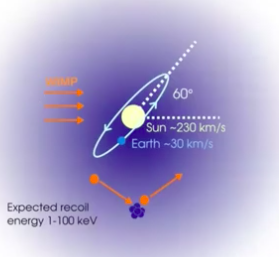
\includegraphics[scale=0.45]{darkmatter1.png}\qquad\qquad\qquad
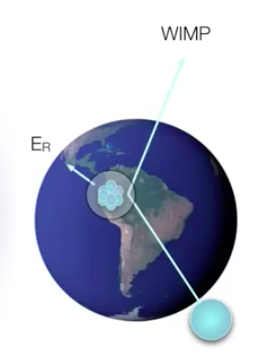
\includegraphics[scale=0.4]{darkmatter2.png}
\end{figure}

One can perform a rough calculation to determine how many dark matter particles we expect to detect:
\begin{itemize}
\item The dark matter density is given experimentally by $\rho = 0.3\ \textrm{GeV}/\textrm{cm}^3$
\item The average velocity of the Sun is given by $\braket{\vec{v}} = 220\ \textrm{km}/\textrm{s}$.
\item We don't know the mass of the dark matter particles, but in the WIMP models we expect that the mass is around $m \approx 100\ \textrm{GeV}$. 
\end{itemize}
We can then determine the \textit{flux} of WIMPs on Earth:
\begin{equation*}
\phi = \frac{\rho}{m} \braket{\vec{v}} \approx 10^5\ \textrm{cm}^{-2}\textrm{s}^{-1}.
\end{equation*}
Thus tens of millions of dark matter particles are flying through your hand every second!


\newpage
One important strategy we can employ in the detection of dark matter is \textit{directionality}. From our position on Earth,  we know that dark matter particles arrive from a \textit{precise direction} in the sky, namely the \textit{Cygnus constellation}. They travel at velocities around $220\ \textrm{km}/\textrm{s}$. When they hit some special nuclei that forms part of our detector, there is an \textit{elastic collision} that results in movement of the nuclei - this is measurable because the nuclei is visible (unlike the WIMP).
\begin{figure}[H]
\centering
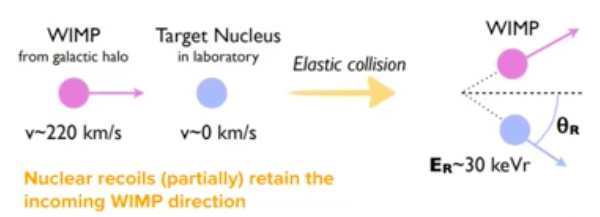
\includegraphics[scale=0.4]{wimpscattering.png}
\end{figure}
If we see nuclei moving in a direction that is compatible with the direction that we expect dark matter to arrive from, this could be evidence of dark matter detection.\\

The direction is very important because there are many other things that can hit a nucleus, and the nucleus can move for other reasons unrelated to dark matter. The general problem is that \textit{whilst the flux of WIMPs is high, the probability of interaction is very low}. In a sensitive detector we expect $1$ event per kilogram per year (compare this with placing a banana near the detector - this causes around $100$ events per kilogram per year, because of the radiation from the potassium in the banana!). Therefore, the experimental challenge is to detect a \textit{tiny signal} over a \textit{large background}.

\minirule

There are some differences between signal and background events. A dark matter signal comprises only \textit{nuclear recoil}, whilst most of the background is comprised of \textit{electron recoil} caused by photon interactions. On the other hand the background does also include nuclear recoil events caused by neutrons, which are similar to WIMP nuclear recoil events.

\begin{figure}[H]
\centering
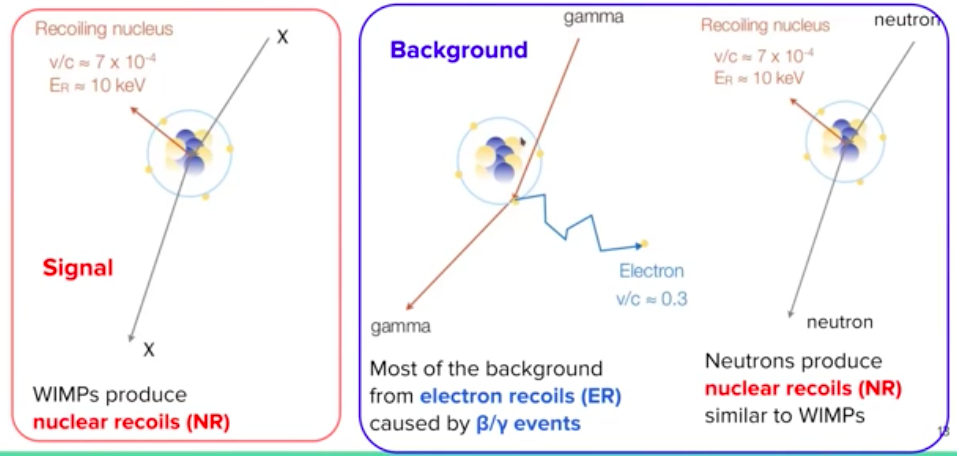
\includegraphics[scale=0.4]{wimprecoil.png}
\end{figure}

There are two main sources of background: 
\begin{enumerate}[label = (\arabic*)]
\item \textit{Cosmic rays}. These are a problem if you would like to do your measurement on the Earth's surface. To mitigate the effect, we can work in underground laboratories.
\item \textit{Environmental radioactivity} (mainly from potassium, uranium and thorium). This comes even from the walls of your lab! To mitigate this effect, we can shield the equipment, and carefully choose materials with low levels of radioactivity in the setup.
\end{enumerate} 



\newpage
\subsection{Dark matter detection with a time projection chamber}
\describesection{Gas tank detection. Images of electron recoil tracks and nuclear recoil tracks. Goal of the school's competition.}
We will now describe in more detail the detection of dark matter via nuclear recoil.\\

The general idea is to us a \textit{gas target}; for example the gas used in the CYGNO experiment, based in Italy, is a mixture of helium $\textrm{He}$ and carbon tetrafluoride $\textrm{CF}_4$. The advantage of using a gas target is that it is not very dense, so the recoiling nucleus can travel several millimetres. This direction can be measured. 

\begin{figure}[H]
\centering
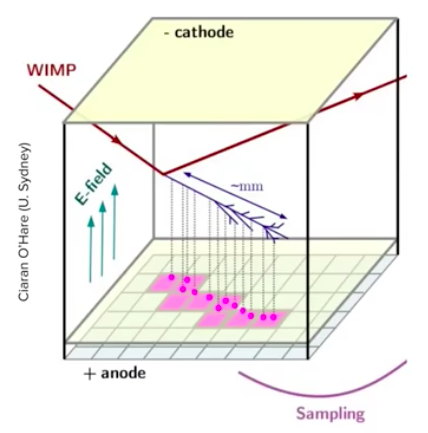
\includegraphics[scale=0.4]{gastank.png}
\end{figure}

The way the measurement works is as follows. Electrons from the struck nucleus are ionised, and an electric field is applied to the detector such that the electrons move towards the \textit{anode} of the detector. The amount of electrons that reach the anode is proportional to the released energy, which implies we can measure energy deposits and their position in the $xy$-plane, giving a 2D projection of the particles' track.\\
Here are some examples of (simulated, cleaned) tracks from electron recoils in the CYGNO experiment:
\begin{figure}[H]
\centering
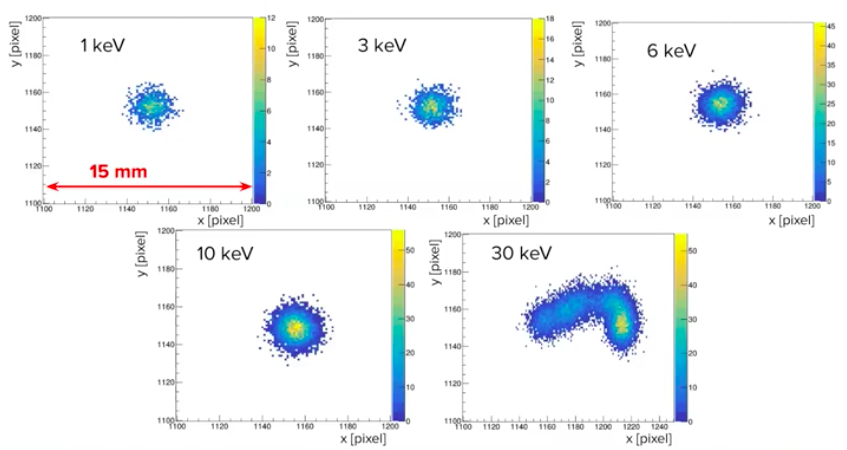
\includegraphics[scale=0.4]{electrontracks.png}
\end{figure}


\newpage
Here are some examples of (simulated, cleaned) tracks from helium recoils in the CYGNO experiment:
\begin{figure}[H]
\centering
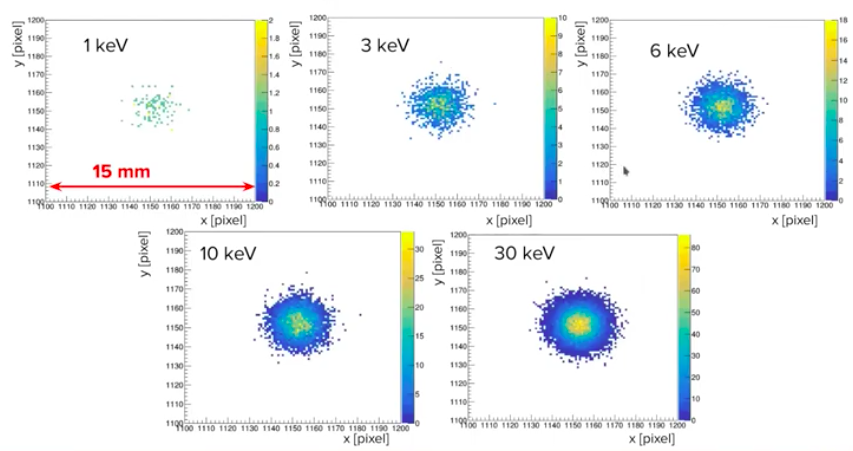
\includegraphics[scale=0.4]{heliumtracks.png}
\end{figure}

As you can see from the figures, there is a somewhat visible difference between electron recoil and helium recoil.\\

When noise is added, the figures become slightly more complicated:

\begin{figure}[H]
\centering
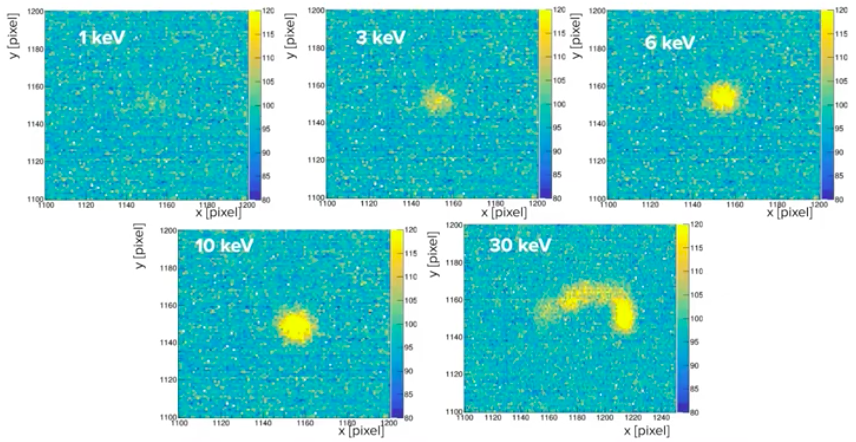
\includegraphics[scale=0.4]{noisyelectrontracks.png}
\end{figure}
For smaller energies it can be difficult by eye to even find the track!

\minirule

The goal of the competition at the school is to devise a machine learning procedure to distinguish between electron recoil (ER) and helium nuclear recoil (NR) in such tracks. The events will have energies ranging from $1$ to $30 \textrm{ keV}$ (the most important energy range for dark matter searches, and also the most challenging region for background rejection), together with a random initial angle. There will be precisely one particle for each image in each case.



\newpage
\part{Introduction to machine learning}
\hrule
\noindent \\
\section{Introduction to supervised learning}

\subsection{Problem setup}
\describesection{Problem setup for supervised learning. Basic examples.}

\begin{framedef}
Consider a set $\mathcal{X}$ of objects and a set of targets $\mathcal{Y}$. Suppose also that there is an unknown function $f : \mathcal{X} \rightarrow \mathcal{Y}$ mapping objects into targets (which may be stochastic - by which we mean the objects and targets are drawn from some joint probability distribution).\\

A \textit{dataset} is a finite collection $D = \{(x_i,f(x_i)) : i=1,...,N\} \subseteq \mathcal{X} \times \mathcal{Y}$. The goal of \textit{supervised learning} is to \textit{approximate $f$ given a dataset $D$} (i.e. learn to recover targets from objects). 
\end{framedef}

\begin{frameex}
\begin{enumerate}[label = (\roman*)]
\item \textbf{Classification of iris flower species.} The objects $\mathcal{X}$ are individual flowers, described by the length and width of their sepals and petals. The targets $\mathcal{Y}$ are the species to which the flowers belong. The mapping $f : \mathcal{X} \rightarrow \mathcal{Y}$ takes a flower to its species (and depends on different shapes of sepals, petals, etc corresponding to the different species). Note this is a \textit{non-deterministic} mapping because the growth of a certain flower is associated with a number of random processes.
\item \textbf{Spam filtering.} The objects $\mathcal{X}$ are emails (sequences of characters). The targets are the categories $\mathcal{Y} = \{\text{spam}, \text{not spam}\}$. The mapping $f : \mathcal{X} \rightarrow \mathcal{Y}$ tells us whether a particular email $x \in \mathcal{X}$ is spam or not, and is again \textit{non-deterministic} (the style and content can vary from author to author).
\item \textbf{CAPTCHA recognition.} The set of objects $\mathcal{X}$ is a set of CAPTCHA images (which are really vectors of pixel level brightness). The set of targets $\mathcal{Y}$ are sequences of characters, relating to the correct word that the CAPTCHA shows. The mapping $f : \mathcal{X} \rightarrow \mathcal{Y}$ is the inverse of the algorithm used to generate the CAPTCHA - this is \textit{almost} deterministic, but depends on the level of distortion (very high distortion can make the map less deterministic).
\item \textbf{Particle identification in a HEP experiment.} The objects $\mathcal{X}$ are particles, described by the detector experiments (e.g. track parameters, calorimeter energy, deposit, etc.). The targets $\mathcal{Y}$ are the types of the particles (e.g. electrons, muons, protons, etc.). The mapping $f : \mathcal{X} \rightarrow \mathcal{Y}$ is the inverse of the physical process generating the detector response (by definition, this is a stochastic process).
\end{enumerate}
\end{frameex}



\newpage
\subsection{Feature types}
\describesection{Features and the design matrix. Numeric, categorical nominal, categorical ordinal and binary features. One-hot encoding.}
Typically the objects in our set $\mathcal{X}$ will have some structure.

\begin{framedef}
Let $\mathcal{X}$, $\mathcal{Y}$ be the sets of objects and targets in a supervised learning problem. Suppose that $\mathcal{X}$ is a collection of \textit{tuples}, so that given a dataset $D \subseteq \mathcal{X} \times \mathcal{Y}$, for each $(x_i,f(x_i)) \in D$ we can write $x_i$ as:
\begin{equation*}
x_i = (x_i^1,x_i^2,...,x_i^d),
\end{equation*}
for some $d$ (which need not be the same for all $x_i \in \mathcal{X}$). We say that $x_i^j$ is a \textit{feature} of the object $x_i$ (note we use the upper index for the \textit{feature}, and the lower index to label the object in the dataset).\\

Many algorithms require that the \textit{dimensionality} $d$ of the data is the same for all objects. In this case, the dataset can be represented by a \textit{design matrix}:
\begin{equation*}
X = \begin{pmatrix} x_1^1 & x_1^2 & \cdots & x_1^d \\ x_2^1 & x_2^2 & \cdots & x_2^d \\ \vdots & \vdots & \ddots & \vdots \\ x_N^1 & x_N^2 & \cdots & x_N^d \end{pmatrix}.
\end{equation*}
The column index corresponds to the features, and the row index corresponds to the position of the object in the dataset.
\end{framedef}

\begin{frameex}
Consider the problem of classifying species of irises. In this case, features might include \textit{sepal length}, \textit{sepal width}, \textit{petal length} and \textit{petal width}. In this case, all of the features are real numbers.\\

Since each flower will have these features, we can describe all objects as $4$-tuples, and hence we can organise the data into a $N \times 4$ design matrix.
\end{frameex}


\begin{framedef}
In general, features $x_i^j$ might be of varying natures. We give special names to some common cases:
\begin{itemize}
\item \textit{Numeric features} take values in (for example) the real numbers. For example sepal length in the classification of iris species, building height, or particle transverse mometnum.
\item \textit{Categorical nominal features} take values in a finite set, with no natural ordering. For example colour, city of birth or particle type.
\item \textit{Categorical ordinal features} take values in a set equipped with a natural order, for example level of education, age, or particles passing loose, medium or tight selection criteria.
\item \textit{Binary features} take values in a set of size $2$, for example $\{\text{true}, \text{false}\}$, $\{0,1\}$, $\{-1,+1\}$. 
\end{itemize}
\end{framedef}

A natural question that arises in the handling of data is how one might convert a categorical nominal feature into a binary or numeric feature (since binary or numeric features can be more easily handled).\\

A na\"{i}ve approach would be to assign each category a number (e.g. red$=1$, green$=2$, etc). However, this introduces an ordering on the feature, which could have a negative effect on learning algorithms later on. 


\newpage
A better solution is \textit{one-hot encoding}:

\begin{framedef}
Let $x_i = (x_i^1,...,x_i^{j-1},x_i^j,x_i^{j+1}, ..., x_i^d)$ be an object in a dataset, and let $x_i^j$ be a categorical nominal feature for the object, taking values in some finite set $S$. A \textit{one-hot encoding} replaces the feature $x_i^j$ with $|S|$ binary features $\{x_i^{j,s} : s \in S\}$ obeying:
\begin{equation*}
x_i^{j,s} = \begin{cases} 0 & \text{if $x_i^j \neq s$,}\\ 1 & \text{if $x_i^j = s$.} \end{cases}
\end{equation*}
The new object then takes the form 
\begin{equation*}
x_i = (x_i^1,...,x_i^{j-1}, x_i^{j,s_1},...,x_i^{j, s_{|S|}}, x^{j+1},...,x_i^d),
\end{equation*}
where $s_i \in S$ are the elements of $S$.
\end{framedef}

\begin{frameex}
Suppose $x$ is a categorical nominal feature taking values in the set $\{\text{red}, \text{blue}, \text{green}\}$. A one-hot encoding of the object is:
\begin{equation*}
(x^{\text{red}}, x^{\text{blue}}, x^{\text{green}}),
\end{equation*}
where $x^{\text{red}} = 0$ if $x \neq \text{red}$, $1$ if $x = \text{red}$, etc.\\

For example, $x = \text{red}$ is replaced by $(1,0,0)$, whilst $x = \text{green}$ is replaced by $(0,0,1)$. 
\end{frameex}

One-hot encoding can also be applied to categorial ordinal features:

\begin{framedef}
Let $x_i = (x_i^1,...,x_i^{j-1},x_i^j,x_i^{j+1}, ..., x_i^d)$ be an object in a dataset, and let $x_i^j$ be a categorical \textit{ordinal} feature for the object, taking values in some finite set $S$ with ordering $<$. Suppose that the elements of $S$ are ordered as $s_1 < s_2 < \cdots < s_{|S|}$. A \textit{one-hot encoding} replaces the feature $x_i^j$ with $|S|$ binary features $\{x_i^{j,s} : s \in S\}$ obeying:
\begin{equation*}
x_i^{j,s} = \begin{cases} 0 & \text{if $s < x_i^j$,}\\ 1 & \text{if $x_i^j \leq s$.} \end{cases}
\end{equation*}
The new object then takes the form 
\begin{equation*}
x_i = (x_i^1,...,x_i^{j-1}, x_i^{j,s_1},...,x_i^{j, s_{|S|}}, x^{j+1},...,x_i^d).
\end{equation*}
\end{framedef}

\begin{frameex}
Suppose $x$ is a categorical ordinal feature taking values in the ordered set $\{\text{bachelors}, \text{masters}, \text{PhD}\}$, with ordering $\text{bachelors} < \text{masters} < \text{PhD}$. A one-hot encoding of the object is:
\begin{equation*}
(x^{\text{bachelors}}, x^{\text{masters}}, x^{\text{PhD}}).
\end{equation*}
For example, $x = \text{bachelors}$ is replaced by $(1,0,0)$, whilst $x = \text{PhD}$ is replaced by $(1,1,1)$. \\

Note that this \textit{retains} the ordering of the original categorical ordinal feature.
\end{frameex}





\newpage
\subsection{Learning algorithms}
\describesection{Definition of a learning algorithm. Loss functions, e.g. least squares error. Examples of $k$ nearest neighbours and linear regression.}
\begin{framedef}
Let $\mathcal{X}, \mathcal{Y}, f$ be the respective objects, targets and function of a supervised learning problem. Given a dataset $D = \{(x_i,f(x_i)) : i=1,2,...,N\} \subseteq \mathcal{X} \times \mathcal{Y}$, a \textit{learning algorithm} $\mathcal{A}$ returns an approximation $\hat{f} = \mathcal{A}(D)$ (which depends on the dataset) to the true function $f$.
\end{framedef}

\begin{framedef}
The \textit{$k$ nearest neighbours algorithm} can be applied when the features of the objects have some notion of distance (i.e. a \textit{metric}). We then define:
\begin{equation*}
\hat{f}(x) = \frac{1}{k} \sum_{i : x_i \in D_{x}^k} f(x_i),
\end{equation*}
where $D_{x}^k$ is the set of $k$ objects in the dataset $D$ closest to $x$.
\end{framedef}

\begin{frameex}
Consider a \textit{classification problem} where the target space $\mathcal{Y}$ consists of only two values. In this case the $k$ nearest neighbours algorithm approximates the function $f : \mathcal{X} \rightarrow \mathcal{Y}$ by:
\begin{equation*}
\hat{f}(x) = \underset{C}{\textrm{argmax}} \sum_{i : x_i \in D_x^k} 1_{\{f(x_i) = C\}},
\end{equation*}
where $1_{\{f(x_i) = C\}}$ is the relevant indicator function. Note that instead of averaging the target, we take the value of $C$ which maximises the sum, either $0$ or $1$.
\end{frameex}

In general, how does one find an algorithm $\mathcal{A}$ giving an approximation $\hat{f} = \mathcal{A}(D)$ to the true mapping function? Many algorithms work by solving an \textit{optimisation task} - namely, minimising a \textit{loss function}:

\begin{framedef}
Let $\hat{f} = \mathcal{A}(D)$ be the approximation to the true mapping function for a supervised learning problem $f : \mathcal{X} \rightarrow \mathcal{Y}$, with dataset $D \subseteq \mathcal{X} \times \mathcal{Y}$ given. A \textit{loss function} is a function $\mathcal{L} : \mathcal{Y} \times \mathcal{Y} \rightarrow \mathbb{R}$, chosen to measure the quality of predictions. The \textit{loss} of our approximation at the point $x_i \in \mathcal{X}$ in the dataset is given by $\mathcal{L}(f(x_i), \hat{f}(x_i))$. 
\end{framedef}

\begin{frameex}
An example of a loss function is \textit{least squares error}, given by $\mathcal{L}(f(x_i),\hat{f}(x_i)) = (f(x_i) - \hat{f}(x_i))^2$, where the target space $\mathcal{Y} = \mathbb{R}$.
\end{frameex}

\begin{framedef}
Given a loss function $\mathcal{L} : \mathcal{Y} \times \mathcal{Y} \rightarrow \mathbb{R}$ for a supervised learning problem, we can obtain an approximation $\hat{f} = \mathcal{A}(D)$ of the true mapping $f : \mathcal{X} \rightarrow \mathcal{Y}$ from a datset $D$ via \textit{loss minimisation}:
\begin{equation*}
\hat{f} = \underset{\tilde{f}}{\textrm{argmin}} \underset{(x_i,f(x_i)) \in D}{\mathbb{E}} \mathcal{L}(f(x_i), \tilde{f}(x_i)),
\end{equation*}
where the $\textrm{argmin}$ is taken over all functions $\tilde{f} : \mathcal{X} \rightarrow \mathcal{Y}$, and the notation $\mathbb{E}$ means the expected value of the loss over the dataset (in the case that the mapping is stochastic, this is important).
\end{framedef}



\newpage
\begin{frameex}
An example is \textit{linear regression}, where we take $\mathcal{X} = \mathbb{R}^d$, $\mathcal{Y} = \mathbb{R}$. In this case, the functions $\tilde{f}$ which could constitute possible mappings $\mathcal{X} \rightarrow \mathcal{Y}$ are restricted to simply be \textit{linear functions}, of the form:
\begin{equation*}
\tilde{f}_{\vec{w},\vec{b}}(\vec{x}) = \vec{w}^T \vec{x} + \vec{b}.
\end{equation*}
Given a dataset $D \subseteq \mathcal{X} \times \mathcal{Y}$ of size $N$, minimising the least squared loss corresponds to determining $\vec{w}, \vec{b}$ such that:
\begin{equation*}
\frac{1}{N}\sum_{i=1,...,N} \left( f(x_i) - \hat{f}_{\vec{w},\vec{b}}(x_i) \right)^2
\end{equation*}
is minimised.
\end{frameex}


\newpage
\subsection{Assumptions about data and model complexity}
\describesection{Training and test data. The curse of dimensionality. Model complexity.}
Given no assumptions about a dataset, there are typically infinitely many solutions to a loss minimisation problem. For example, if we wish to interpolate a finite set of points for a one-dimensional function, infinitely many curves will perfectly minimise the loss (defined in this case as the sum of the distances between the curve and the point at each point).\\

To combat these, we introduce the concept of \textit{test data}:

\begin{framedef}
A set of \textit{test data} is an independent dataset drawn from the same population as the dataset used to construct the solution of our loss minimisation problem (this original set is called the \textit{training data}).
\end{framedef}

We then demand that our expected loss on the whole population (i.e. both the test and training data) is minimised. 

\begin{frameex}
Consider a linear interpolation problem in $\mathbb{R}^d$ which we solve both with the $k$ nearest neighbour algorithm, and with linear regression. Suppose the true dependence is also linear.\\

It turns out that if we validate our approaches using a test set, the error on the test set for $k$ nearest neighbour and linear regression agree well for lower dimensions $d$, but $k$ nearest neighbour becomes much worse for larger numbers of dimensions.\\

This feature is called the \textit{curse of dimensionality} - as the number of dimensions of the feature space grows, the data becomes very sparse, and the $k$ nearest neighbour approach begins to fail. In this case, to keep the error low, the number of training points would have to increase exponentially with the dimension.\\

The reason we get the distinction is that the two algorithms have different assumptions:
\begin{itemize}
\item The $k$ nearest neighbour (kNN) approach assumes that \textit{similar objects have similar targets}.
\item The linear regression approach assumes that \textit{targets are linear in features}.
\end{itemize}
In this case, both assumptions are correct, but linearity is much stronger which allows us to fight the curse of dimensionality. \\

In particular, imposing assumptions about the data \textit{restricts the possible function space of solutions $\tilde{f}$} for the loss minimisation problem:
\begin{equation*}
\hat{f} = \underset{\tilde{f}}{\textrm{argmin}} \underset{(x_i,f(x_i)) \in D}{\mathbb{E}} \mathcal{L}(f(x_i), \tilde{f}(x_i)),
\end{equation*}
Linearity is a much stronger constraint than kNN imposes (kNN allows for a much more flexible functional form), restricting the space of functions much more. Sometimes these restrictions help us to \textit{overcome the curse of dimensionality}. 
\end{frameex}

\begin{framedef}
The \textit{complexity} of a model refers to the heuristic size of the function space over which we minimise in the loss minimisation problem. A larger complexity means a larger function space, whilst a smaller complexity means a smaller function space.
\end{framedef}



\newpage
In general, changing the model complexity can allow us to find the `sweet spot' where expected loss on both the training and test data sets is minimised:

\begin{figure}[H]
\centering
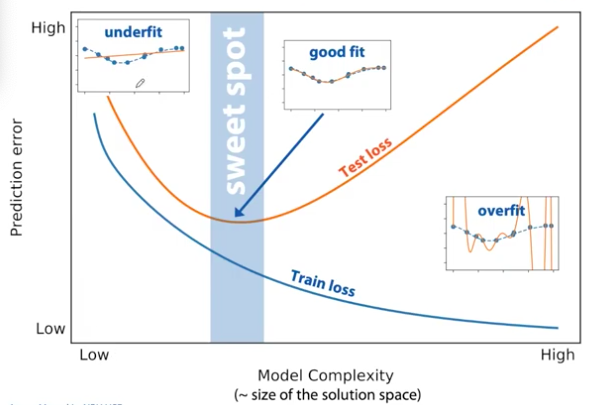
\includegraphics[scale=0.5]{traintest.png}
\end{figure}

The goal is to find the \textit{right level of limitations} - not too strict, not too loose.




\newpage
\section{Linear models}
\subsection{Linear models and linear regression}
\describesection{Linear models and examples. `Hidden power' of linear models via feature transformation. Examples of loss functions: MSE, MAE, MAPE and MSLE.}
\begin{framedef}
A \textit{linear model} is a model $\hat{f}(x)$ which is linear in its input (note this assumes a vector space structure on both the objects and targets). 
\end{framedef}

\begin{frameex}
Examples include:
\begin{itemize}
\item Linear regression, for example $\hat{f}(\vec{x}) = \pmb{\theta}^T \vec{x}$.
\item Classification, for example $\hat{f}(\vec{x}) = 1_{\{\pmb{\theta}^T\vec{x} > 0\}}$. This is non-linear as a function, but divides the target space by a line.
\end{itemize}
\end{frameex}

Linear models have a \textit{hidden power}. Problems which appear linearly inseparable (i.e. cannot be solved with linear models) can be made into problems which are tractable with linear models by \textit{transforming the features}. As an example, the data on the left below can be made linearly separable by introducing a new feature based on the sum of the squares of the coordinates of the points:

\begin{figure}[H]
\centering
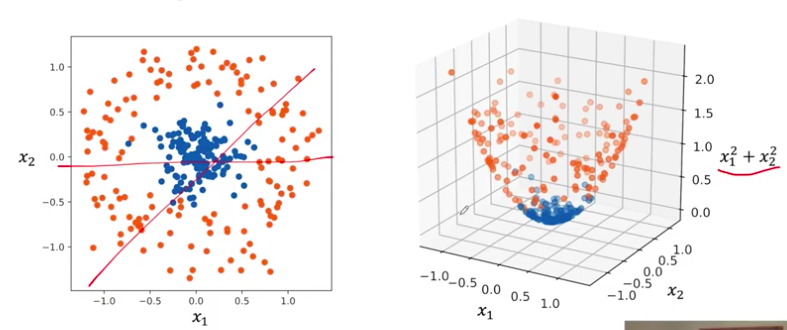
\includegraphics[scale=0.5]{hiddenlinear.png}
\end{figure}

Now a hyperplane separates the blue and orange sets.\\

In general, linear models motivate the construction of \textit{deep models}. Neural networks are just linear models with \textit{activation functions} between them (effecting some transformation). Thus better understanding linear models will help us understand deep neural networks. \\

We have already introduced linear regression as a linear model. Here, we update the notation:
\begin{framedef}
The \textit{model prediction} is $\hat{f}_{\pmb{\theta}}(\vec{x}) = \pmb{\theta}^T \vec{x}$, where $\pmb{\theta} \in \mathbb{R}^d$ is our \textit{parameter vector}, $\vec{x} \in \mathcal{X} \subseteq \mathbb{R}^d$ is our \textit{features vector}, and:
\begin{equation*}
\frac{1}{N} \sum_{i=1,...,N} \left( f(\vec{x}_i) - \hat{f}_{\pmb{\theta}}(\vec{x}_i) \right)^2
\end{equation*}
is our mean squared error loss, given a dataset. We wish to minimise this over $\pmb{\theta}$.
\end{framedef}


\newpage
Other loss functions are available. For example:
\begin{itemize}
\item \textbf{Mean absolute error (MAE).} This is given by:
\begin{equation*}
\frac{1}{N} \sum_{i=1,...,N} \left|f(\vec{x}_i) - \hat{f}_{\pmb{\theta}}(\vec{x}_i)\right|.
\end{equation*}
This grows linearly for large errors, rather than quadratically like mean squared error loss. In particular, it doesn't penalise large errors as much as mean squared error loss - it might be more suitable if there are outliers in your data which you do not wish to be biased against.
\item \textbf{Mean absolute percentage error (MAPE).} This is given by:
\begin{equation*}
\frac{1}{N} \sum_{i=1,..,N} \left| \frac{f(\vec{x}_i) - \hat{f}_{\pmb{\theta}}(\vec{x}_i)}{f(\vec{x}_i)} \right|.
\end{equation*} 
\item \textbf{Mean squared logarithmic error (MSLE).} This is given by:
\begin{equation*}
\frac{1}{N} \sum_{i=1,...,N} \left( \log(f(\vec{x}_i) + 1) - \log(\hat{f}_{\pmb{\theta}}(\vec{x}_i) + 1) \right)^2.
\end{equation*}
The $1$'s are there just to allow zero values of the targets. 
\end{itemize}
Both MAPE and MSLE provide a means of computing \textit{relative error}, so are useful when the targets span through a large range of magnitudes.\\

In general, applying different loss functions are also related to different assumptions about the data. A different loss function might be more suitable to a particular dataset.





\newpage
\subsection{Analytic solution}
\describesection{Analytic solution for linear models. Ill-conditioning and flat directions. Bias terms.}
Recall that earlier we defined the design matrix $X$, a matrix with rows given by the objects and columns given by the features. We can use this to rewrite the mean squared error loss as:
\begin{equation*}
\mathcal{L}_{\text{MSE}} = \frac{1}{N} \sum_{i=1,...,N} \left( f(\vec{x}_i) - \pmb{\theta}^T \vec{x}_i \right)^2 = \frac{1}{N} || \vec{y} - X \pmb{\theta} ||^2,
\end{equation*}
where $\vec{y} = (f(\vec{x}_1),...,f(\vec{x}_N))^T$.\\

To minimise this function, we can ignore the $1/N$ as it plays no role. Thus we wish to minimise $||\vec{y} - X\pmb{\theta}||^2$ over $\pmb{\theta}$. Analytically, the requirements are:
\begin{equation*}
\frac{\partial}{\partial \pmb{\theta}} \mathcal{L}_{\text{MSE}} = \vec{0}, \qquad \text{the matrix }\frac{\partial^2}{\partial \theta_i \partial \theta_j} \mathcal{L}_{\text{MSE}}\text{ of second derivatives should be positive definite.}
\end{equation*}
The first condition ensures we have an extremum, the second condition ensures that extremum is a minimum.

\begin{frameprop}
If the columns of $X$ are linearly independent, the solution to the above minimisation problem is $\pmb{\theta} = (X^TX)^{-1} \vec{y}$.\\

\textit{Proof:} Note that in general, the matrix $X^TX$ is always \textit{positive semi-definite}, since:
\begin{equation*}
\vec{v}^T X^T X\vec{v} = ||X\vec{v}||^2 \geq 0
\end{equation*}
for arbitrary $\vec{v}$. We see it is \textit{precisely} positive definite when the columns of $X$ are linearly independent (imagine the expression $X\vec{v}$ to be a linear combination of the columns of $X$). This additionally implies $X$ is invertible (e.g. all its eigenvalues are positive).\\

We can now consider the optimisation problem. The first derivative of $\mathcal{L}_{\text{MSE}}$ is easily computed:
\begin{equation*}
\frac{\partial}{\partial \pmb{\theta}} \mathcal{L}_{\text{MSE}} = \frac{1}{N}\frac{\partial}{\partial \pmb{\theta}} (\vec{y} - X \pmb{\theta})^T (\vec{y} - X\pmb{\theta}) = -\frac{2}{N}X^T (\vec{y} - X\pmb{\theta}) = \vec{0}.
\end{equation*}
This implies that $X^T \vec{y} - X^T X \pmb{\theta} = \vec{0}$. Since $X^TX$ is invertible, we can compute the solution:
\begin{equation*}
\pmb{\theta} = (X^T X)^{-1} X^T \vec{y}.
\end{equation*}
To check that this is a minimum, we must look at the second derivative. We find that the matrix of second derivatives is precisely:
\begin{equation*}
2X^TX.
\end{equation*}
In particular, this matrix is positive definite by the above. \qedsymbol
\end{frameprop}

In practice, there may be some linear dependence of the columns of $X$ (i.e. there may be some `feature correlations'). This affects the invertibility of the matrix $X^TX$ - we get \textit{flat directions}, and hence multiple solutions to the problem.

\begin{figure}[H]
\centering
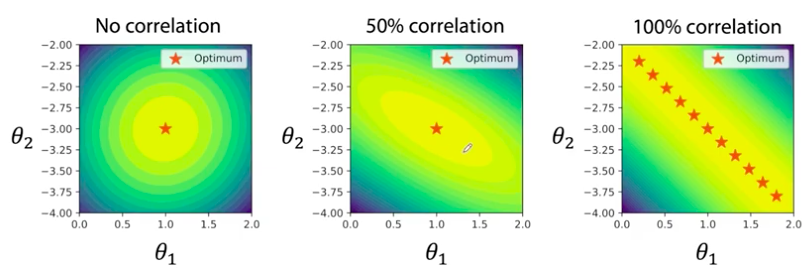
\includegraphics[scale=0.3]{featurecorrelations.png}
\end{figure}


\newpage
In the above we also assumed that our model took the form $\hat{f}_{\pmb{\theta}}(\vec{x}) = \pmb{\theta}^T \vec{x}$ for ease of calculation, but actually we can consider the more general linear model $\hat{f}_{\pmb{\theta}}(\vec{x}) = \pmb{\theta}^T \vec{x} + \theta_0$, where the term $\theta_0$ is called the \textit{bias term}. There is no need to redo any calculations here; we simply add a constant feature to the design matrix to account for this:
\begin{equation*}
X = \begin{pmatrix} x_1^1 & x_1^2 & \cdots & x_1^d \\ x_2^1 & x_2^2 & \cdots & x_2^d \\ \vdots & \vdots & \ddots & \vdots \\ x_N^1 & x_N^2 & \cdots & x_N^d \end{pmatrix} \qquad \rightarrow \qquad X =\begin{pmatrix} 1 & x_1^1 & x_1^2 & \cdots & x_1^d \\ 1 & x_2^1 & x_2^2 & \cdots & x_2^d \\ \vdots & \vdots & \vdots & \ddots & \vdots \\ 1 & x_N^1 & x_N^2 & \cdots & x_N^d \end{pmatrix}
\end{equation*}
Now when we multiply $X\pmb{\theta}$, one of the parameters will play the role of the bias term.

\begin{figure}[H]
\centering
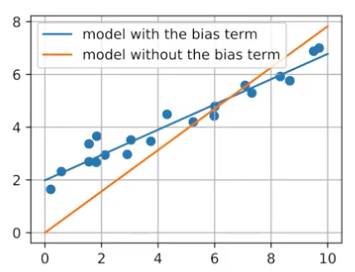
\includegraphics[scale=0.4]{biasterm.png}
\end{figure}





\newpage
\subsection{Numerical and stochastic optimisation: gradient descent}
\describesection{The gradient and its geometric interpretation. The gradient descent algorithm; convex functions. Overfitting and early stopping. Stochastic gradient descent.}
We have now discussed the analytic solution for the mean squared error loss minimisation problem in the context of a linear model. However, most loss functions do not allow an analytic solution, so it is important to discuss numerical solutions.\\

We being with some revision of the \textit{gradient}. Recall that the gradient of a scalar function on $\mathbb{R}^d$ is given by:
\begin{equation*}
\nabla f(\vec{x}) = \left( \frac{\partial f}{\partial x_1}(\vec{x}), ..., \frac{\partial f}{\partial x_d}(\vec{x}) \right).
\end{equation*}
The gradient always points in the \textit{direction of greatest increase} of the function. Hence if we start at a point, and move in the opposite direction to the gradient, we will get closer to a local minimum - this aids optimisation.\\

Let us formalise this:
\begin{framedef}
Given a smooth function $f : \mathbb{R}^d \rightarrow \mathbb{R}$ and an initial point $\vec{x}^{(0)}$, we define a recursive sequence of points via:
\begin{equation*}
\vec{x}^{(k)} = \vec{x}^{(k-1)} - \alpha \nabla f(\vec{x}^{(k-1)}),
\end{equation*}
where $\alpha \in \mathbb{R}_{> 0}$ is a constant called the \textit{learning rate}. This construction is called \textit{gradient descent iteration}.

\begin{figure}[H]
\centering
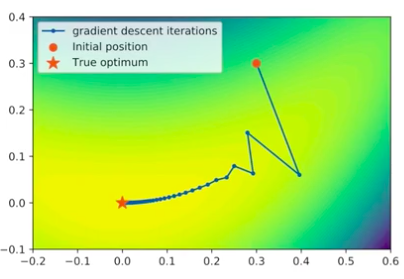
\includegraphics[scale=0.3]{gradientdescent.png}
\end{figure}
\end{framedef}

It is possible to show that:
\begin{frameprop}
For smooth, \textit{convex} functions with a single minimum $\vec{x}^* \in \mathbb{R}^d$, we have:
\begin{equation*}
f(\vec{x}^{(k)}) - f(\vec{x}^*) = O\left( \frac{1}{k} \right),
\end{equation*}
i.e. as we take more and more points, we approach the true minimum of the function.
\end{frameprop}

Gradient descent may also be applied to non-convex functions, but we may reach a minimum which is not \textit{global}, and the result may \textit{depend on the starting point}. 

\begin{figure}[H]
\centering
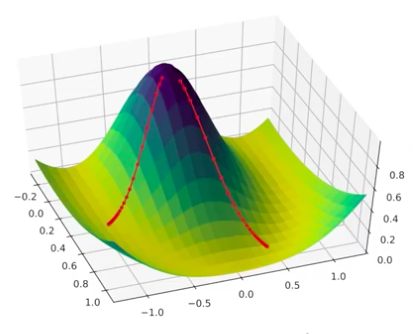
\includegraphics[scale=0.3]{nonconvex.png}
\end{figure}


\newpage
A useful property of gradient descent is that it can be used for \textit{regularisation} when our loss function is ill-defined; for example, when our $X^TX$ matrix above is not invertible (or not stably invertible). \\

In such cases, the true minimum typically has very large parameter values. These often correspond to \textit{overfitting}. To avoid this, we can start from a point where our initial parameters are \textit{small} and we can stop the gradient descent early (this is called \textit{early stopping}). This will typically be a better solution than the true minimum.

\begin{figure}[H]
\centering
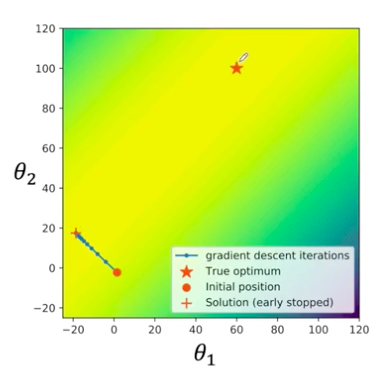
\includegraphics[scale=0.4]{regularisation.png}
\end{figure}

There is an important modification to the gradient descent algorithm called \textit{stochastic gradient descent}. Recall that in machine learning we typically optimise loss functions which are averages over some set of objects:
\begin{equation*}
L = \frac{1}{N} \sum_{i=1,...,N} \mathcal{L}\left(f(x_i), \hat{f}_{\theta}(x_i) \right).
\end{equation*}
For large $N$, gradient descent is computationally inefficient and may be unfeasible in terms of memory consumption. Stochastic gradient descent deals with this problem:
\begin{framedef}
Given a function $\hat{f}_{\pmb{\theta}} : \mathcal{X} \rightarrow \mathcal{Y}$ which depends on a parameter $\pmb{\theta} \in \mathbb{R}^d$, a starting point $\pmb{\theta}^{(0)}$, and a set of objects $x_1,...,x_N \in \mathcal{X}$, we define a recursive sequence of points as follows:
\begin{itemize}
\item At step $k$ of the process, pick some $l_k \in \{1,...,N\}$ at random.
\item Define:
\begin{equation*}
\pmb{\theta}^{(k)} = \pmb{\theta}^{(k-1)} - \alpha \nabla_{\pmb{\theta}} \mathcal{L}\left(f(x_{l_k}), \hat{f}_{\pmb{\theta}^{(k-1)}}(x_{l_k}) \right).
\end{equation*}
\end{itemize}
This is called \textit{stochastic gradient descent iteration}.
\end{framedef}

In the case of a smooth convex function, stochastic gradient descent also leads you to the unique minimum, but at a slower rate of $O(1/\sqrt{k})$ instead. This \textit{can} be improved by `batching' and other tricks.



\newpage
\subsection{Feature expansion}
\describesection{General description of feature transformation. Examples of polynomial feature transformations.}
Let us now see how linear models can be made more powerful by transforming their features.

\begin{framedef}
Given a design matrix $X$ of dimension $N \times d$, a \textit{feature transformation} via the function $\Phi : \mathbb{R}^d \rightarrow \mathbb{R}^{d'}$ is the induced map of the design matrix:
\begin{equation*}
X = \begin{pmatrix} x_1^1 & x_1^2 & \cdots & x_1^d \\ x_2^1 & x_2^2 & \cdots & x_2^d \\ \vdots & \vdots & \ddots & \vdots \\ x_N^1 & x_N^2 & \cdots & x_N^d \end{pmatrix} \qquad \rightarrow \qquad \Phi(X) =\begin{pmatrix} \Phi^1(x_1^1,...,x_1^d) & \cdots & \Phi^{d'}(x_1^1,...,x_1^d) \\ \Phi^1(x_2^1,...,x_2^d) & \cdots & \Phi^{d'}(x_2^1,...,x_2^d) \\ \vdots & \ddots & \vdots \\ \Phi^1(x_N^1,...,x_N^d) & \cdots & \Phi^{d'}(x_N^1,...,x_N^d)\end{pmatrix}
\end{equation*}
Finding good functions $\Phi$ to transform with is called \textit{feature engineering}. It is an important part of machine learning and requires a deep understanding of the underlying problem and the data.
\end{framedef}

\begin{frameex}
(\textbf{Polynomial features.}) Consider trying to fit the curve $y = x + \frac{1}{2}x^2$. This cannot be solved using only linear regression; a single line will not work.
\begin{figure}[H]
\centering
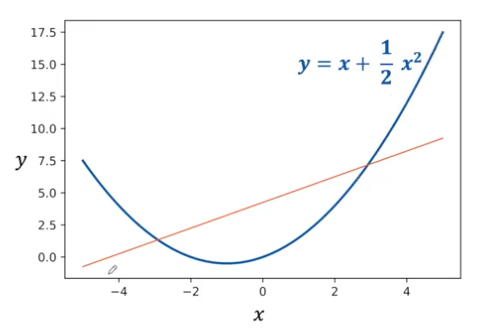
\includegraphics[scale=0.3]{quadvslinear.png}
\end{figure}
However, we can introduce a new feature via a feature transformation. Let $(x_1, x_2) = (x,x^2)$. Then in the new feature space, a linear estimate is really an estimate of the form $\hat{f}(\vec{x}) = \theta_1 x_1 + \theta_2 x_2 = \theta_1 x + \theta_2 x^2$, which facilitates fitting.
\begin{figure}[H]
\centering
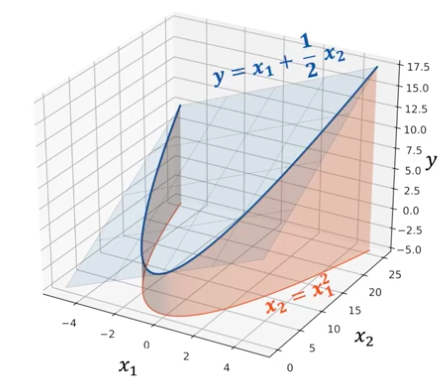
\includegraphics[scale=0.3]{featuretrans.png}
\end{figure}
\end{frameex}



\begin{frameex}
(\textbf{Polynomial features - general case}) Let $(x_i^1,x_i^2,...,x_i^d)$ be the original features of a dataset. We introduce as new features all unique multiplicative combinations of the form:
\begin{equation*}
(x_i^1)^{p_1}(x_i^2)^{p_2} ... (x_i^d)^{p_d},
\end{equation*}
where $p_1 + p_2 + \cdots + p_m \leq p$ (with $p$ the degree we expect to work).
\end{frameex}







\newpage
\section{Classification with linear models}

\subsection{Classification with linear regression}
\describesection{Classification problems; na\"{i}ve approach with MSE loss. Better approach with smooth approximations to $0$-$1$ loss.}
Consider a classification problem, with two classes, as shown below:
\begin{figure}[H]
\centering
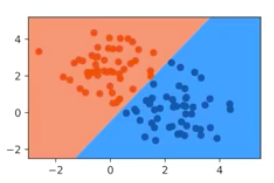
\includegraphics[scale=0.7]{classificationproblem.png}
\end{figure}
Since there are only two classes, we can assign numeric values to the classes - for our convenience, we choose $y = +1$ for one class (the `positive' class) and $y = -1$ for the other class (the `negative' class)\\

We can try to predict these targets with a linear model. To do so, we solve a linear regression problem using the model $\hat{y}_{\pmb{\theta}}(\vec{x}) = \pmb{\theta}^T\vec{x}$. To obtain the classified function, we then simply take the sign of the result:
\begin{equation*}
\hat{f}(\vec{x}) = \textrm{sign}(\hat{y}(\vec{x})).
\end{equation*}

This may seem like a reasonable approach, but you can face problems. Consider the following set:
\begin{figure}[H]
\centering
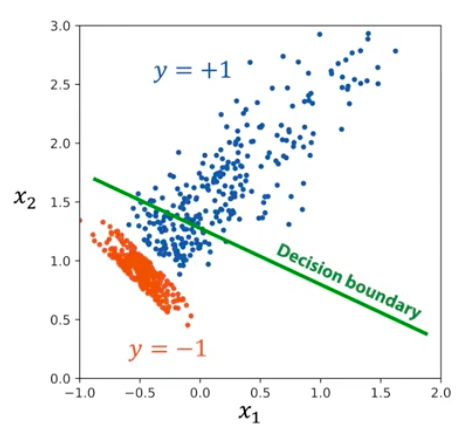
\includegraphics[scale=0.4]{decisionboundary.png}
\end{figure}
Here, the MSE loss makes the model avoid high errors, at the price of \textit{pushing the decision boundary} towards the class with higher spread.




\newpage

Therefore, we might try to use a different loss function. A good first example is \textit{$0$-$1$ loss}.
\begin{framedef}
For the above classification problem, we define the \textit{$0$-$1$ loss by}:
\begin{equation*}
\mathcal{L}_{0\text{-}1} = \frac{1}{N} \sum_{i=1,...,N} 1_{\{\pmb{\theta}^T \vec{x}_i y_i < 0\}}
\end{equation*}
where $y_i \in \{-1,+1\}$. We call $M = \pmb{\theta}^T \vec{x} y$ the \textit{margin}. When $M > 0$, we have a \textit{correct} classification, but when $M < 0$ we have an \textit{incorrect} classification. The higher the magnitude of $M$, the further an object is from the decision boundary. \\

The sum computes the number of times our linear regression misclassifies a point. 
\end{framedef}

Unfortunately, the resulting $0$-$1$ loss function is a piecewise constant function of $\pmb{\theta}$:
\begin{equation*}
\centering
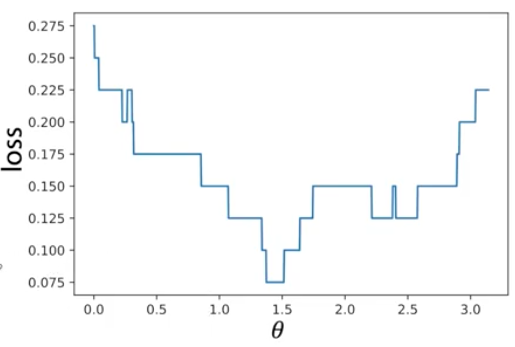
\includegraphics[scale=0.4]{01loss.png}
\end{equation*} 
This means that we cannot use \textit{gradient descent} to minimise our loss (of course, there are other methods - we will discuss them later).\\

Instead of using $0$-$1$ loss then, we could replace the sharp `step' function described by the loss by a \textit{differentiable upper bound}:
\begin{figure}[H]
\centering
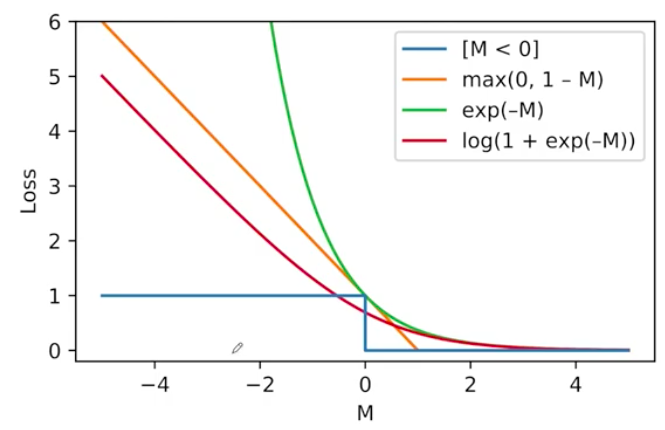
\includegraphics[scale=0.4]{upperbound.png}
\end{figure}
Examples are shown in the above figure (the red line can be scaled to be above the step function). We will discuss the red line (\textit{log loss}) in much more detail as we discuss \textit{logistic regression}.



\newpage
\subsection{Logistic regression}
\describesection{Logistic regression from class probabilities and maximum log likelihood. The sigmoid function and the logistic regression loss function.}
Let's depart from the discussion above, and approach things from a different way to start with. Consider modelling the \textit{class probabilities}: we introduce a function $\hat{f}_{\pmb{\theta}}(\vec{x})$ that gives the probability of an object $\vec{x}$ being in the class $y=+1$, so that:
\begin{equation*}
\mathbb{P}(y=+1 | \vec{x}) = \hat{f}_{\pmb{\theta}}(\vec{x}), \qquad \mathbb{P}(y=-1 | \vec{x}) = 1 - \hat{f}_{\pmb{\theta}}(\vec{x}).
\end{equation*}
How can we optimise such a model? We can fit with the \textit{maximum log likelihood}.\\

Recall that the \textit{likelihood} is defined by:
\begin{equation*}
\text{likelihood} = \prod_{i=1,...,N} \mathbb{P}(y_i|\vec{x}_i) = \prod_{i=1,...,N} \left( 1_{\{y_i = +1\}} \hat{f}_{\pmb{\theta}}(\vec{x}_i) + 1_{\{y_i = -1\}} \left(1 - \hat{f}_{\pmb{\theta}}(\vec{x}_i) \right) \right).
\end{equation*}
Maximising the logarithm likelihood allows us to obtain the best values of the parameter $\pmb{\theta}$:
\begin{equation*}
\pmb{\theta} = \underset{\pmb{\theta}}{\textrm{argmax}} \sum_{i=1,...,N} \left( 1_{\{y_i = +1\}} \log\left(\hat{f}_{\pmb{\theta}}(\vec{x}_i) \right) + 1_{\{y_i = -1\}} \log\left( 1 - \hat{f}_{\pmb{\theta}}(\vec{x}_i) \right) \right).
\end{equation*}
Note that the indicator functions can be moved out of the logarithm because only one of them is equal to $1$ at a time.\\

Once we have fitted the parameter values, we can for example predict the class the \textit{highest probability} for each $\vec{x} \in \mathcal{X}$ in the object space. More generally, we could not just choose the highest probability class but try to use a probability threshold that is suitable for our problem.


\minirule

Let's try to relate this back to linear models now. We need to ask: how can we map a linear model output to a probability value in $[0,1]$? A common choice is the \textit{sigmoid function}:
\begin{framedef}
The \textit{sigmoid function} is defined by:
\begin{equation*}
\sigma(x) = \frac{1}{1 + e^{-x}}.
\end{equation*}
It has the useful property that $1 - \sigma(x) = \sigma(-x)$. 
\end{framedef}
This can be applied to the above example, since we can define:
\begin{equation*}
\mathbb{P}(y=+1|\vec{x}) = \sigma(\pmb{\theta}^T \vec{x}). 
\end{equation*}
where $\pmb{\theta}^T \vec{x}$ is our linear model. The linear model $\pmb{\theta}^T \vec{x}$ then has the meaning of \textit{log odds ratio} between the two classes:
\begin{equation*}
\log\left( \frac{\mathbb{P}(y = +1 | \vec{x})}{\mathbb{P}(y = -1 | \vec{x})} \right) = \log\left( \frac{1}{1 + e^{-\pmb{\theta}^T \vec{x}}} \cdot \frac{1 + e^{-\pmb{\theta}^T \vec{x}}}{e^{-\pmb{\theta}^T \vec{x}}} \right) = \pmb{\theta}^T \vec{x}.
\end{equation*}
Therefore to bring everything together, we use the negative log likelihood as our loss function:
\begin{align*}
\mathcal{L} &= - \sum_{i=1,...,N} \left( 1_{\{y_i = +1\}} \log\left(\hat{f}_{\pmb{\theta}}(\vec{x}_i) \right) + 1_{\{y_i = -1\}} \log\left( 1 - \hat{f}_{\pmb{\theta}}(\vec{x}_i) \right) \right) \\[1.5ex]
&= \sum_{i=1,...,N} \left( 1_{\{y_i = +1\}} \log\left(\sigma(\pmb{\theta}^T \vec{x}_i)\right) + 1_{\{y_i = -1\}} \log\left(  \sigma(-\pmb{\theta}^T \vec{x}_i) \right) \right)\\[1.5ex]
&= - \sum_{i=1,...N} \log\left( \sigma(\pmb{\theta}^T \vec{x}_i y_i ) \right) = \sum_{i=1,...N} \log\left(1 + e^{-\pmb{\theta}^T \vec{x}_i y_i} \right).
\end{align*}
This is the same as the `red' example we used above when we discussed upper bounds on $0$-$1$ loss. We can apply gradient descent or stochastic gradient descent here.


\newpage
Applying to the dataset above, the decision boundary is in the correct place with logistic regression:
\begin{figure}[H]
\centering
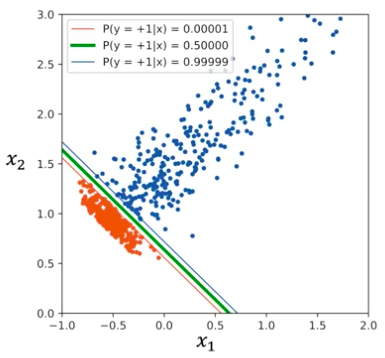
\includegraphics[scale=0.4]{decisionboundary2.png}
\end{figure}
Note that when the classes are linearly separable as above, for any correct decision boundary, mapping $\pmb{\theta} \rightarrow C \cdot \pmb{\theta}$ for some $C > 1$ keeps the boundary at the same place, yet improves the loss. The ideal fit is when the sigmoid turns into a step function (at infinitely large $\pmb{\theta}$.\\

If the classes overlap however, the predicted class probability changes smooth, and the loss has a finite minimum.

\begin{figure}[H]
\centering
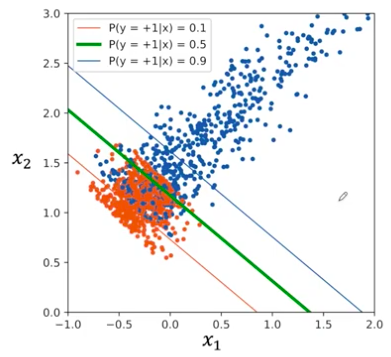
\includegraphics[scale=0.4]{decisionboundary3.png}
\end{figure}



\newpage
\subsection{Multinomial logistic regression}
\describesection{Logistic regression for many classes using class probabilities; symmetry of the parameters. The multinomial logistic regression loss function.}
Similarly to the binary case, we can model the class probabilities when there are more classes than $2$. Let's model the \textit{unnormalised} class probabilities as:
\begin{equation*}
\tilde{\mathbb{P}}(y = k | \vec{x}) = \exp\left( \pmb{\theta}_k^T \vec{x} \right),
\end{equation*}
where we now have $K$ parameter vectors, $k = 1,...,K$. The normalised probabilities can be straightforwardly obtained:
\begin{equation*}
\mathbb{P}(y = k | \vec{x}) = \frac{\exp\left( \pmb{\theta}_k^T \vec{x} \right)}{\sum_{k'=1,...,K} \exp(\pmb{\theta}_{k'}^T \vec{x})}
\end{equation*}
This function is called \textit{softmax} and is commonly used in neural networks.\\

Note that there is a transformational symmetry here: transforming $\pmb{\theta}_k \mapsto \pmb{\theta}_k + \vec{v}$ by some constant vector $\vec{v}$ does not affect the normalised probability. We have:
\begin{equation*}
\tilde{\mathbb{P}}(y = k | \vec{x}) = e^{\pmb{\theta}_k^T\vec{x}} \rightarrow e^{\vec{v}^T \vec{x}} \cdot e^{\pmb{\theta}_k^T \vec{x}} = e^{\vec{v}^T \vec{x}} \cdot \tilde{\mathbb{P}}(y = k | \vec{x}).
\end{equation*}
The remaining exponential cancels out in the ratio in the normalised probabilities. Therefore, we have some extra degree of freedom, which we are free to choose - we can therefore set $\pmb{\theta}_K = \vec{0}$ without loss of generality for example (i.e. we set the last parameter to zero). We are left with $K-1$ parameter vectors.\\

Individual linear outputs $\pmb{\theta}_k^T \vec{x}$ now have the meaning of \textit{log odds ratio} between the classes $k$ and $K$:
\begin{equation*}
\log\left( \frac{\mathbb{P}(y = k | \vec{x})}{\mathbb{P}(y = K | \vec{x})} \right) = \log\left( \frac{\tilde{\mathbb{P}}(y = k | \vec{x})}{\tilde{\mathbb{P}}(y = K | \vec{x})} \right) = \log\left( \frac{e^{\pmb{\theta}_k^T \vec{x}}}{e^0} \right) = \pmb{\theta}_k^T \vec{x}.
\end{equation*}
Putting everything into the negative log likelihood function, we again get our loss function:
\begin{equation*}
\mathcal{L} = - \sum_{i=1,...,N} \log\left( \frac{\exp(\pmb{\theta}_{y_i}^T \vec{x}_i)}{1 + \sum_{k' = 1,...,K-1} \exp\left( \pmb{\theta}_{k'}^T \vec{x}_i \right)}\right),
\end{equation*}
where $\pmb{\theta}_K = \vec{0}$. Again, this can be optimised \textit{numerically} using gradient descent or stochastic gradient descent.


\newpage
\subsection{Multiclass classification: general approach}
\describesection{One-versus-rest multiclass classification. Comparison with logistic regression.}
In fact, you are not limited to use logistic regression for multiclass classification - you are able to use any linear model.\\

For a problem with $K$ classes, introduce $K$ predictors:
\begin{equation*}
\hat{f}_k(\vec{x}) : \mathcal{X} \rightarrow \mathbb{R}
\end{equation*}
for $k = 1,..., K$ each of which outputs a corresponding \textit{class score}. We can use this to predict the class with the \textit{highest score}:
\begin{equation*}
\hat{y}_i = \underset{k}{\textrm{argmax}} \hat{f}_k(\vec{x}_i).
\end{equation*}
For example, any binary linear classification model can be converted to a multiclass classification with the \textit{one-versus-rest} strategy:
\begin{itemize}
\item For each class $k$ train a binary model $\hat{f}_k(\vec{x}) = \pmb{\theta}^T_{(k)}\vec{x}$ separating the given class from all others, $\hat{y}^{\text{one-vs-rest}}_{(k)} = \textrm{sign}(\hat{f}_k(\vec{x}))$. 
\item Use the outputs of $\hat{f}_k$ as class scores for multiclass classification:
\begin{equation*}
\hat{y}_i = \underset{k}{\textrm{argmax}} \hat{f}_k(\vec{x}_i).
\end{equation*}
\end{itemize}

\begin{frameex}
In the following three-class classification, the one-versus-rest splits given by using the appropriate binary classifiers are shown below:
\begin{figure}[H]
\centering
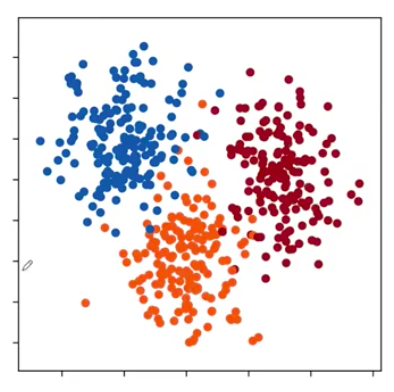
\includegraphics[scale=0.4]{onevsrest1.png}
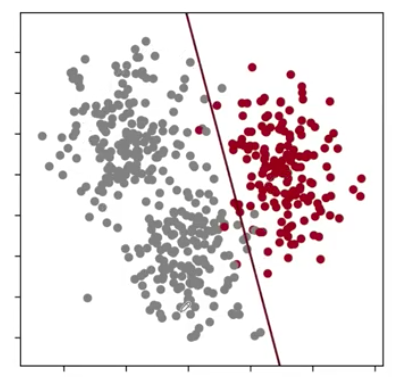
\includegraphics[scale=0.4]{onevsrest2.png}
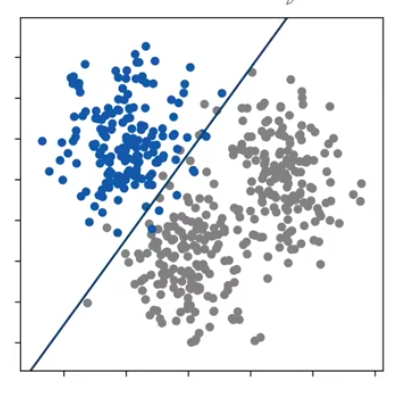
\includegraphics[scale=0.4]{onevsrest3.png}
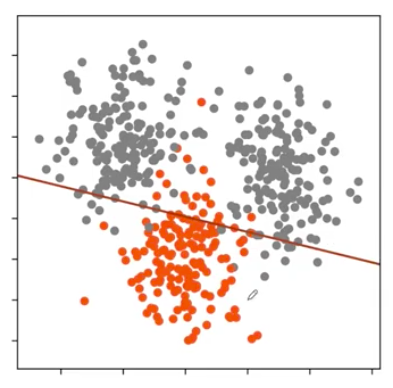
\includegraphics[scale=0.4]{onevsrest4.png}
\end{figure}

\newpage
The resulting decision boundaries can be built up as follows:
\begin{figure}[H]
\centering
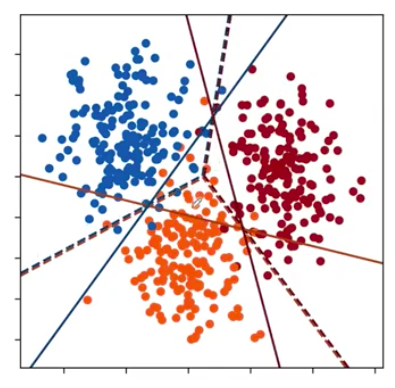
\includegraphics[scale=0.4]{decisionboundaries2.png}
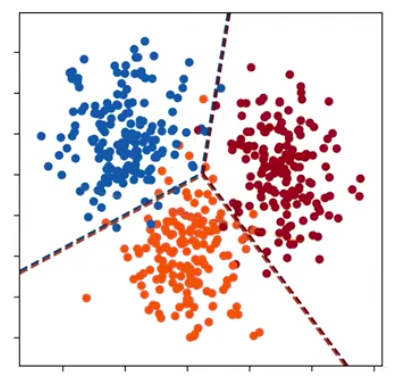
\includegraphics[scale=0.4]{decisionboundaries3.png}
\end{figure}
\end{frameex}

Is the one-vs-rest approach better than multinomial logistic regression however? Some problems are not linearly separable, so one-vs-rest results in biased class probabilities whilst logistic regression is still quite accurate:
\begin{figure}[H]
\centering
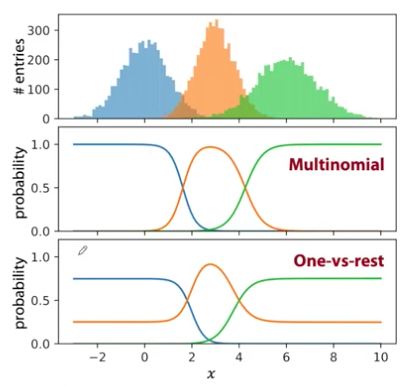
\includegraphics[scale=0.6]{logisticvsonevsrest.png}
\end{figure}





\newpage
\section{Model regularisation}

\subsection{The problem of overfitting}
\describesection{Recap of overfitting and test set.}
Overfitting is the tendency of a model to adjust to random fluctuations in the data. This can be detected by a model making poor predictions on the \textit{test set}.

\begin{figure}[H]
\centering
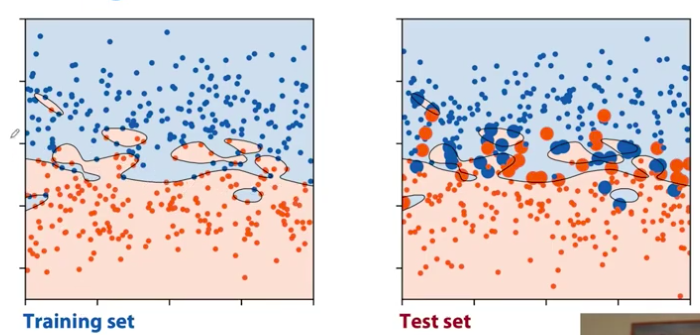
\includegraphics[scale=0.4]{overfitting.png}
\end{figure}

Recall that we need to use a model complexity such that we don't underfit, and we don't overfit - we need to find the `sweet spot' in between.

\minirule

\subsection{Prediction error decomposition}
\describesection{Decomposition of error sources: model variance, bias, and irreducible error. The bias-variance tradeoff. Bias and variance of linear models.}
Before talking about regularisation, let's discuss the prediction error of a model. Assume that there's the following unknown relation between features and targets:
\begin{equation*}
y = f(x) + \epsilon,
\end{equation*}
where $\epsilon$ is some random noise, $\mathbb{E}[\epsilon] = 0$ and $\textrm{Var}[\epsilon] = \sigma_{\epsilon}^2$. Let's denote a training set as $\tau$. We want to study the \textit{expected squared error} for the model $\hat{f}_{\tau}$ trained on the dataset $\tau$:
\begin{equation*}
\textrm{exp.sq.err}(x) = \underset{\tau, y}{\mathbb{E}}\left[ (\hat{f}_{\tau}(x) - y )^2 | x \right].
\end{equation*}
The target $y$ is sampled independently of the training set.\\

We can rewrite this expression in the following form, by adding and subtracting the `prediction of the expected model' and the `ground truth' $f(x)$ (without the noise):
\begin{align*}
\textrm{exp.sq.err}(x) &= \underset{\tau, y}{\mathbb{E}}\left[ (\hat{f}_{\tau}(x) - y )^2 | x \right]\\[1.5ex]
&= \underset{\tau,y}{\mathbb{E}}\left[ \left( (\hat{f}_{\tau}(x) - \underset{\tau'}{\mathbb{E}}[\hat{f}_{\tau'}(x)]) + (\underset{\tau'}{\mathbb{E}}[\hat{f}_{\tau'}(x)] - f(x)]) + (f(x) - y)\right)^2 \bigg| x\right]\\[1.5ex]
&= \underset{\tau}{\mathbb{E}}\left[ \left(\hat{f}_{\tau}(x) - \underset{\tau'}{\mathbb{E}}[\hat{f}_{\tau'}(x)] \right)^2\right] + \left( \underset{\tau'}{\mathbb{E}}[\hat{f}_{\tau'}(x)] - f(x) \right)^2 + \underset{y}{\mathbb{E}}[(f(x) - y)^2 | x].
\end{align*}
In the final step, we have expanded everything and used the fact that the cross-term expectation are $0$ (this follows from the fact that $\tau, y$ are sampled independently).


\newpage
\noindent The remaining terms have important interpretations:
\begin{itemize}
\item The first term is the \textit{variance of the model}. It quantifies how `unstable' the model is with respect to the noise in the training data.
\item The second term is the \textit{squared bias}. It is how much the `expected model' differs from the ground truth.
\item The third term is the \textit{irreducible error}. Substituting the true dependence $y$, we find it is just given by $\sigma_{\epsilon}^2$. This error cannot be eliminated.
\end{itemize}
The first two errors on the other hand, can be removed by changing the model. Typically there's a \textit{tradeoff} between the two types of errors:
\begin{figure}[H]
\centering
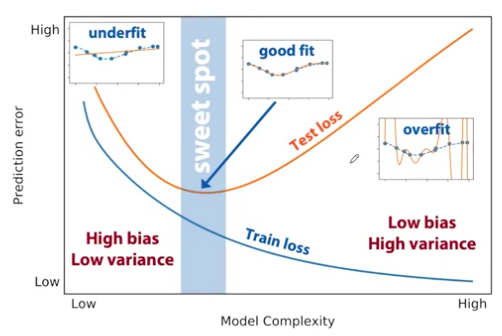
\includegraphics[scale=0.4]{biasvariancetradeoff.png}
\end{figure}
For low model complexity, the \textit{bias} is high because we are artificially simplifying the model - it doesn't depend much on the data (it has `low variance'). The opposite is true for high model complexity. This tradeoff is called the \textit{bias-variance tradeoff}.

\begin{frameex}
Let's compute the bias and variance of a linear model. For each expectation $\mathbb{E}$ with respect to $\tau$, we will assume that the features are \textit{fixed}, i.e. $X_{\tau} = X$ (i.e. the design matrix is constant), and only the target vector $y_{\tau}$ is random. This simplification allows us to analytically compute the result.\\

Recall the solution for the linear regression model with the MSE loss:
\begin{equation*}
\hat{f}_{\tau}(\vec{x}) = \pmb{\theta}_{\tau}^T\vec{x}, \qquad \pmb{\theta}_{\tau} = (X^TX)^{-1} X^T \pmb{y}_{\tau}.
\end{equation*}
The \textit{bias term} from the above error decomposition is:
\begin{equation*}
\textrm{bias}(\vec{x}) = \underset{\tau}{\mathbb{E}}[\hat{f}_{\tau}(\vec{x})] - f(\vec{x}) = \underset{\tau}{\mathbb{E}}\left[ \vec{x}^T (X^TX)^{-1}X^T \vec{y}_{\tau} \right] - \vec{x}^T \pmb{\theta}_{\text{true}}
\end{equation*}
We also assume that the true dependence is indeed linear, i.e. $f(\vec{x}) = \vec{x}^T \pmb{\theta}_{\text{true}}$ for some $\pmb{\theta}_{\text{true}}$.\\

Since $X$ does not depend on the sampling dataset $\tau$, we can move lots of things out of the expectation, leaving:
\begin{equation*}
\vec{x}^T (X^TX)^{-1}X^T \underset{\tau}{\mathbb{E}}[\vec{y}_{\tau} - \vec{x}^T \pmb{\theta}_{\text{true}} = \vec{x}^T (X^TX)^{-1} X^TX \pmb{\theta}_{\text{true}} - \vec{x}^T \pmb{\theta}_{\text{true}} = \vec{x}^T \pmb{\theta}_{\text{true}} - \vec{x}^T \pmb{\theta}_{\text{true}} = 0.
\end{equation*}
Hence we see that the linear regression model is \textit{unbiased}, provided the true dependence is linear.


\newpage
Now let's consider the \textit{variance term}:
\begin{equation*}
\textrm{variance}(\vec{x}) = \underset{\tau}{\mathbb{E}} \left[ \left(\hat{f}_{\tau}(\vec{x}) - \underset{\tau'}{\mathbb{E}}[\hat{f}_{\tau'}(\vec{x})]\right)^2 \right].
\end{equation*}
It can be shown that:
\begin{equation*}
\textrm{variance}(\vec{x}) = \sigma_{\epsilon}^2 \vec{x}^T (X^TX)^{-1} \vec{x},
\end{equation*}
so that the variance error component is a \textit{quadratic form}, defined by the $(X^TX)^{-1}$ matrix. We can diagonalise $X^TX$ giving:
\begin{equation*}
\textrm{variance}(\vec{x}) = \sigma_{\epsilon}^2 \tilde{\vec{x}}^T \Lambda^{-1} \tilde{\vec{x}},
\end{equation*}
where $\Lambda = \textrm{diag}\{\lambda_1,...,\lambda_d\}$ is the diagonal matrix of eigenvalues of $X^TX$. This means that \textit{small eigenvalues amplify the model variance}. This happens when $X^TX$ is ill-defined, e.g. when the features are correlated.

\begin{figure}[H]
\centering
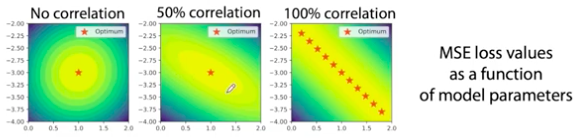
\includegraphics[scale=0.4]{linearvariance.png}
\end{figure}
\end{frameex}

In a high variance model, we expect that a small perturbation data will lead to a large change in the prediction.


\minirule


\subsection{Regularisation}
\describesection{Regularisation methods: $L2$ regularisation, $L1$ regularisation, and elastic net regression. Comparison of methods; sparsity vs weight-sharing.}
How can we reduce the variance of a model? If only we could \textit{increase the eigenvalues} of the matrix $X^TX$. In fact, we can do this manually:
\begin{equation*}
X^TX \rightarrow X^TX + \alpha I,
\end{equation*}
for $\alpha > 0$, with $I$ a unit $d \times d$ matrix. This is called \textit{$L2$ regularisation}.\\

In this case, we change the solution to:
\begin{equation*}
\hat{f}_{\tau}(\vec{x}) = \vec{x}^T (X^TX + \alpha I)^{-1} X^T \vec{y}_{\tau}.
\end{equation*}
Now the model is \textit{no longer biased}. We \textit{increased bias to reduce variance} (we no longer get zero for the bias term of this model.
\begin{figure}[H]
\centering
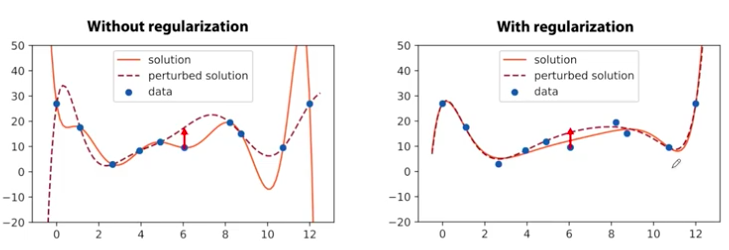
\includegraphics[scale=0.4]{L2regularisation.png}
\end{figure}



\newpage
By regularising the model, we increase the training loss and decrease the test loss. This improves the \textit{generalisability} of the model.

\begin{figure}[H]
\centering
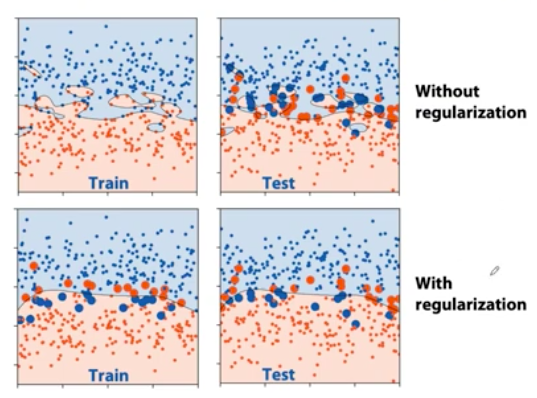
\includegraphics[scale=0.4]{generalisability.png}
\end{figure}

In order to understand this trick better, let's reverse engineer the loss function it optimises. We have the solution $\hat{f}_{\tau}(\vec{x}) = \vec{x}^T (X^T X + \alpha I)^{-1} X^T \vec{y}_{\tau}$, so the $\pmb{\theta}_{\tau}$ vector should be given by:
\begin{equation*}
\pmb{\theta}_{\tau} = (X^TX + \alpha I)^{-1} X^T \pmb{y}_{\tau}.
\end{equation*}
Regrouping the terms, we have:
\begin{equation*}
(XT^X + \alpha I)\pmb{\theta}_{\tau} = X^T \pmb{y}_{\tau} \qquad \Rightarrow \qquad X^T (X\pmb{\theta}_{\tau} - \vec{y}_{\tau}) + \alpha \pmb{\theta}_{\tau} = \vec{0}.
\end{equation*}
In fact, this is the equation $\partial \mathcal{L} / \partial \pmb{\theta}_{\tau} = \vec{0}$ for the loss function:
\begin{equation*}
\mathcal{L} = ||X\pmb{\theta}_{\tau} - \vec{y}_{\tau}||^2 + \alpha || \pmb{\theta}_{\tau}||^2.
\end{equation*}
This explains the origin of the term \textit{$L2$ regularisation}. The model minimises the MSE loss with an \textit{$L2$ penalty theorem} (this model is also called \textit{ridge regression}).\\

There are other similar regularisation methods:
\begin{itemize}
\item \textit{$L2$ regularisation} or \textit{ridge regression} takes as the loss function $\mathcal{L} = ||X \pmb{\theta}_{\tau} - \vec{y}_{\tau}||^2 + \alpha || \pmb{\theta}_{\tau}||^2$.
\item \textit{$L1$ regularisation} or \textit{lasso regularisation} takes as the loss function $\mathcal{L} = ||X \pmb{\theta}_{\tau} - \vec{y}_{\tau}||^2 + \alpha||\pmb{\theta}_{\tau}||_1$ (where $|| \cdot ||_1$ denotes the $L1$ norm.
\item \textit{Elastic net regression} is a combination of the two:
\begin{equation*}
\mathcal{L} = ||X\pmb{\theta}_{\tau} - \vec{y}_{\tau}||^2 + \alpha || \pmb{\theta}_{\tau}||^2 + \beta || \pmb{\theta}_{\tau}||_{1}.
\end{equation*}
\end{itemize}

The introduction of regularisation methods drive the parameters towards smaller values, yet they \textit{induce different properties} of the solution.

\begin{figure}[H]
\centering
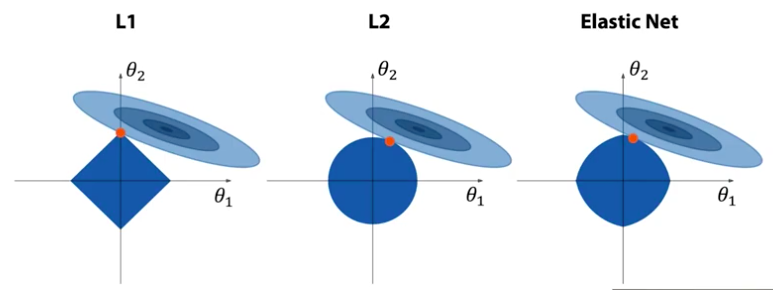
\includegraphics[scale=0.4]{diffregularisations.png}
\end{figure}


\newpage
For example, the $L1$ regularisation term has unit ball given by a diamond in $\theta_1, \theta_2$ space (i.e. the surface where $||\pmb{\theta}||_{1} = 1$). It's quite likely that among all the points at the perimeter of the diamond (where the penalty term does not change), the intersection is most likely at the coordinate axes. This means that this loss tends to \textit{sparsify the solution} - it tends to set some parameters to zero.\\

For the $L2$ regularisation, we instead have \textit{weight sharing} - it uniformly drags the values of the parameters towards zero.\\

The elastic net is a compromise between the two approaches.


\minirule

\subsection{Probabilistic view}
\describesection{Relationship of regularisation to probabilities and maximum likelihood.}
Let's revisit our assumption about the data, $y = f(x) + \epsilon$. Let's now assume that the label noise is \textit{normally distributed}, $\epsilon \sim \mathcal{N}(0,\sigma_{\epsilon}^2)$. This means that the targets, given the objects, are also normally distributed:
\begin{equation*}
y|x \sim \mathcal{N}(f(x), \sigma_{\epsilon}^2).
\end{equation*}
We want our model $\hat{f}_{\theta}(x)$ to fit the true dependence $f(x)$, i.e. we define a \textit{probabilistic model}:
\begin{equation*}
y|x \sim \mathcal{N}(\hat{f}_{\theta}(x),\sigma_{\epsilon}^2),
\end{equation*}
where the mean of the normal distribution is described by our function.\\

Our model can be fitted with the maximum likelihood approach:
\begin{equation*}
L = \prod_{i=1,...,N} \mathcal{N}(y_i | \hat{f}_{\theta}(x_i), \sigma_{\epsilon}^2).
\end{equation*}
Maximising this with respect to $\theta$ is equivalent to minimising the negative log likelihood,
\begin{gather*}
-\log(L) = \sum_{i=1,...,N} \log(\mathcal{N}(y_i | \hat{f}_{\theta}(x_i), \sigma_{\epsilon}^2)) = - \sum_{i=1,...,N} \left[ \log\left( \exp\left( - \frac{(y_i - \hat{f}_{\theta}(x_i) )^2}{2 \sigma_{\epsilon}^2} \right) \right) - \log(\sqrt{2 \pi} \sigma_{\epsilon}^2) \right] \\[1.5ex]
= C \cdot \sum_{i=1,...,N} (y_i - \hat{f}_{\theta}(x_i))^2 + \text{constant}.
\end{gather*}
Thus we just get MSE loss! Thus MSE loss is equivalent to modelling the probability with a normal label noise.\\

You can do similar tricks for other loss functions and show that different probabilistic models lead to different loss functions.




\newpage

\subsection{Bayesian view}
\describesection{Relationship of regularisation to Bayesian priors.}
In the Bayesian view, we treat both data $(X,y)$ and model parameters ($\theta$) as random variables. We estimate the parameter distribution given the observed data via Bayes' rule:
\begin{equation*}
p(\theta | X,y) = \frac{p(y | \theta,X) p(\theta)}{\displaystyle \int \left( p(y | \theta,X) p(\theta) \right) \ d\theta}
\end{equation*}
We assume that $\theta, X$ are independent variables here. Here, $p(\theta)$ is our prior knowledge about the model parameters (our belief about how they are distributed before we see any data). The function $p(y | \theta, X)$ is our likelihood function. The distribution $p(\theta | X,y)$ is called the \textit{posterior distribution}, and is our knowledge about the model after seeing data. The denominator is called `evidence' (the probability of observing the data when the parameter uncertainty is integrated out). \\

To get some estimate of the parameter, we can calculate the \textit{maximum a posteriori} (where we ignore the denominator since is it is integrated over $\theta$ - the maximum is the same as the maximum of the numerator):
\begin{equation*}
\hat{\theta} = \underset{\theta}{\textrm{argmax}}\ p(y | \theta, X) p(\theta) = \underset{\theta}{\textrm{argmin}}\left[ - \log(p(y | \theta, X) - \log(p(\theta)) \right]
\end{equation*}
Similarly, the maximum is the same as the minimum negative log likelihood. The term $\log(p(\theta))$ is called a \textit{regularising} term.

\begin{frameex}
Suppose we model the data with a normal distribution $y|x \sim \mathcal{N}(\hat{f}_{\theta}(x), \sigma_{\epsilon}^2)$. Suppose the prior is normal too $\theta \sim \mathcal{N}(0, \sigma_{\theta}^2 I)$, where $I$ is the unit matrix so that the parameters are uncorrelated. Then maximum a posteriori estimate corresponds to minimising the following loss:
\begin{equation*}
\mathcal{L} = -\log(p(y|\theta,X)) - \log(p(\theta)) = C_1 \sum_{i=1,...,N} (\hat{f}_{\theta}(x_i) - y_i)^2 + C_2 || \theta||^2 + \text{constant}.
\end{equation*}
In other words a normal prior is equivalent to $L2$ regularisation of the parameters.
\end{frameex} 

Choosing different priors will lead to different regularisation of the parameters.





\newpage
\section{Quality metrics for regression and classification}

\subsection{Quality metrics for regression models}
\describesection{Effect of outliers.}
Consider a dataset described by design matrix $X$ and target values $\vec{y}$, and a linear regression model:
\begin{equation*}
\hat{\vec{y}} = X\vec{w},
\end{equation*}
where $\vec{w}$ are the parameters (weights) of the model (previously denoted as $\pmb{\theta}$). Our goal is to \textit{measure the quality} of this model - in other words, estimate how close predictions $\hat{\vec{y}}$ are to the real target values. This is measured by a \textit{loss function}, also called a \textit{quality metric} in this section of the course.\\ 

We have already seen some examples of quality metrics: for example, mean squared error (MSE) and mean absolute error (MAE). Sometimes MSE is replaced by \textit{root mean squared error} (RMSE):
\begin{equation*}
\sqrt{\frac{1}{N} \sum_{i=1}^{N} (\hat{y}_i - y_i)^2}.
\end{equation*} 
With these metrics, it can be hard to tell if a model is good: for example, if RMSE$=1$, the model quality can be different for mean target values of $\overline{y} = 100$ and $\overline{y} = 1$.\\

Another popular metric is MAPE, which we also saw before. It is defined by:
\begin{equation*}
\frac{100}{N} \sum_{i=1}^{N} \left| \frac{\hat{y}_i - y_i}{y_i} \right|.
\end{equation*}
It measures the relative error of the prediction. It is easy to understand the quality of the model, but it is sensitive to the $y$ scale.\\

Two other quality metrics arE:
\begin{itemize}
\item \textbf{Relative square error (RSE).} This is given by:
\begin{equation*}
\sqrt{\frac{\displaystyle \sum_{i=1}^{N} (y_i - \hat{y}_i)^2}{\displaystyle \sum_{i=1}^{N} (y_i - \overline{y})^2}}.
\end{equation*}
This metric measures how the average square error differs from the squared standard deviation of the real target values.
\item \textbf{Relative absolute error (RAE).} This is given by:
\begin{equation*}
\frac{\displaystyle \sum_{i=1}^{N} |y_i - \hat{y}_i|}{\displaystyle \sum_{i=1}^{N} |y_i - \overline{y}|}.
\end{equation*}
Similarly, this metric measures how the average absolute error of the model differs from the the median value of the real target values.
\end{itemize}
The main advantage of these metrics is that they are robust to the scale of the target values $y$.


\newpage
The final quality metric we will consider is \textit{root mean squared logarithmic error} (RMSLE), which we also saw before:
\begin{equation*}
\sqrt{\frac{1}{N} \sum_{i=1}^{N} \left( \log(y_i + 1) - \log(\hat{y}_i + 1) \right)^2}.
\end{equation*}
It is similar to root mean square error, but uses logarithmic values instead. It is used in cases when the target changes by several orders of magnitude - in such cases, the other quality metrics will measure quality less accurately.

\begin{frameex}
Consider the linear regression shown below:
\begin{figure}[H]
\centering
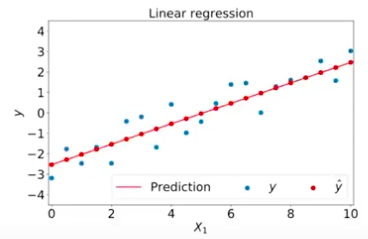
\includegraphics[scale=0.4]{qualitycomparison1.png}
\end{figure}
Computing all of the quality metrics in this case, we have:
\begin{figure}[H]
\centering
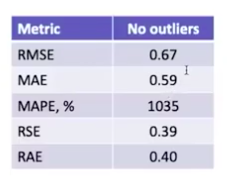
\includegraphics[scale=0.4]{qualitycomparison2.png}
\end{figure}
Note that MAPE fails because of the $y$ scale, and the fact that some $y_i$ are close to zero.\\

Now consider adding a single outlier to the dataset:
\begin{figure}[H]
\centering
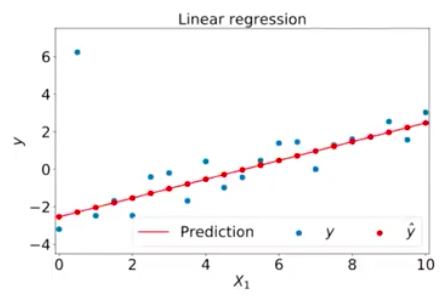
\includegraphics[scale=0.4]{qualitycomparison3.png}
\end{figure}


\newpage
The outlier significantly affects the metrics:
\begin{figure}[H]
\centering
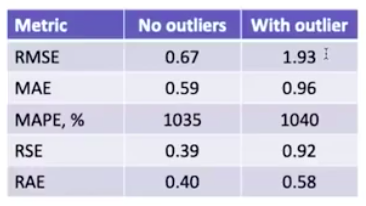
\includegraphics[scale=0.4]{qualitycomparison4.png}
\end{figure}
However, we note that MAE and RAE are the most robust against the addition of the outlier.
\end{frameex}

\minirule

\subsection{Quality metrics for classification models}
Consider a binary classification problem with a data sample and a classifier (into two classes `positive' and `negative'), as shown in the figure. We use a logistic regression model to find the decision boundary.
\begin{figure}[H]
\centering
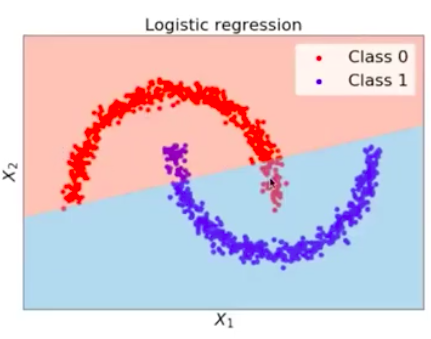
\includegraphics[scale=0.4]{classifierquality.png}
\end{figure}
The goal is to measure the quality of the classifier, i.e. to estimate how well it separates objects of different classes.\\

To measure the model's quality, we introduce a \textit{confusion matrix}:

\begin{framedef}
A \textit{confusion matrix} is a matrix of the form:
\begin{equation*}
\begin{pmatrix} \text{TP} & \text{FN} \\ \text{FP} & \text{TN} \end{pmatrix}.
\end{equation*}
The element TP represents the number of objects which are positive and are correctly predicted as positive (\textit{true positives}). The element FN represents the number of objects which are positive and are incorrectly predicted as negative (\textit{false negatives}).\\

The element FP represents the number of objects which are negative and are incorrectly predicted as positive (\textit{false positives}). The element TN represents the number of objects which are negative and are correctly predicted as negative (\textit{true negatives}).


\newpage
In the example above, we have the following assignments:
\begin{figure}[H]
\centering
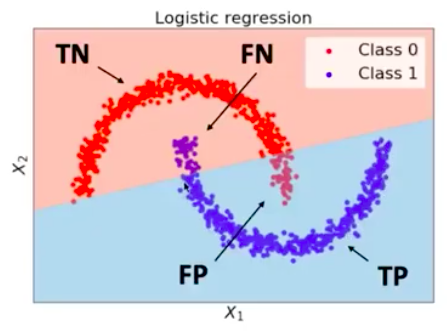
\includegraphics[scale=0.4]{confusionmatrix.png}
\end{figure}
We also define some additional quantities:
\begin{itemize}
\item The number of all positives is $\text{Pos} = \text{TP} + \text{FN}$.
\item The number of all negatives is $\text{Neg} = \text{TN} + \text{FP}$.
\item The number of all positive predictions is $\text{PosPred} = \text{TP} + \text{FP}$.
\item The number of all negative predictions is $\text{NegPred} = \text{TN} + \text{FN}$.
\end{itemize}
\end{framedef}

Using these quantities, we can define different quality metrics. The first metric we define is \textit{accuracy}:

\begin{framedef}
The \textit{accuracy} of a classifier is defined by:
\begin{equation*}
\text{Accuracy} = \frac{\text{TP} + \text{TN}}{\text{TP} + \text{FN} + \text{TN} + \text{FP}} = \frac{\text{TP} + \text{TN}}{\text{Pos} + \text{Neg}}.
\end{equation*}
A complementary quality metric is \textit{error rate}, defined by:
\begin{equation*}
\text{Error rate} = 1 - \text{Accuracy}.
\end{equation*}
These metrics are symmetric and measure quality of classification of both classes equally.
\end{framedef}




\newpage
Other metrics measure how well a classifier identifies positive objects only (i.e. they are asymmetric). Examples include:
\begin{framedef}
\begin{itemize}
\item \textit{Precision} of a classifier is defined by:
\begin{equation*}
\text{Precision} = \frac{\text{TP}}{\text{TP} + \text{FP}} = \frac{\text{TP}}{\text{PosPred}}.
\end{equation*}
\item \textit{Recall} of a classifier is defined by:
\begin{equation*}
\text{Recall} = \frac{\text{TP}}{\text{TP} + \text{FN}} = \frac{\text{TP}}{\text{Pos}}.
\end{equation*}
\item The $F_1$-\textit{score} of a classifier is the harmonic mean of precision and recall, defined by:
\begin{equation*}
F_1 = \frac{2 \cdot \text{Precision} \cdot \text{Recall}}{\text{Precision} + \text{Recall}}.
\end{equation*}
\end{itemize}
\end{framedef}


\begin{frameex}
Consider the classifier example we showed at the start of this section:
\begin{figure}[H]
\centering 
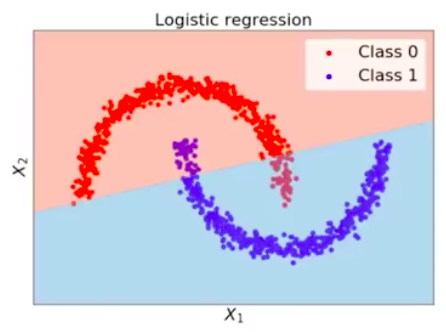
\includegraphics[scale=0.4]{classcomparison.png}
\end{figure}
Computing all of the above metrics on this example, we find:
\begin{figure}[H]
\centering
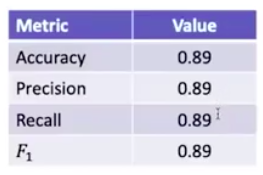
\includegraphics[scale=0.4]{classcomparison2.png}
\end{figure}
All them metrics give the same value in this case, because of the symmetry of the problem. Later we will see other cases.
\end{frameex}



\newpage
Recall that when we did classification problems with logistic regression earlier, we could also have based our ideas on \textit{probabilities}. If an object has a probability $p$ of being in the positive class, we predict it to have value $1$ if $p \geq 0.5$ and value $0$ if $p < 0.5$.\\

The probability in the above example is distributed as a gradient instead of a hard cutoff like the decision boundary:

\begin{figure}[H]
\centering
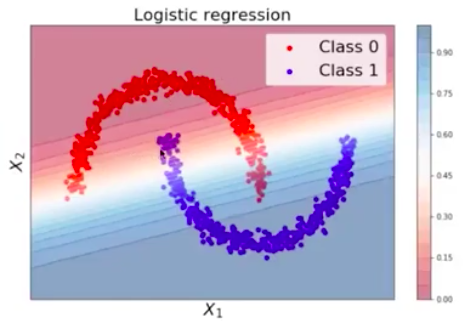
\includegraphics[scale=0.35]{classifierprobability.png}
\end{figure}

We can use these probabilities to define quality metrics.

\begin{framedef}
The \textit{receiver operating characteristic curve} (ROC curve) is a curve relating the \textit{true positive rate} $\text{TPR}(\mu)$ and the \textit{false positive rate} $\text{FPR}(\mu)$ for different `thresholds' $\mu$ of the predicted probabilities $p$. We make the following definitions first:
\begin{itemize}
\item The \textit{true positive rate} is defined by:
\begin{equation*}
\text{TPR}(\mu) = \frac{1}{\text{Pos}} \sum_{i \in \text{Pos}} 1_{\{p_i \geq \mu\}} = \frac{\text{TP}(\mu)}{\text{Pos}},
\end{equation*}
where $\text{TP}(\mu)$ is the number of true positives which have predicted probability of being positive greater than $\mu$.
\item The \textit{false positive rate} is defined by:
\begin{equation*}
\text{FPR}(\mu) = \frac{1}{\text{Neg}} \sum_{i \in \text{Neg}} 1_{\{p_i \geq \mu\}} = \frac{\text{FP}(\mu)}{\text{Neg}},
\end{equation*}
where $\text{FP}(\mu)$ is the number of false positives which have predicted probability of being positive greater than $\mu$.
\end{itemize}
The ROC curve is the curve in the $\text{TPR}, \text{FPR}$ plane parametrised by the threshold $\mu$.
\end{framedef}

\begin{frameex}
For our example above, with the `gradient of probabilities' shown in the figure, the ROC curve looks like:
\begin{figure}[H]
\centering
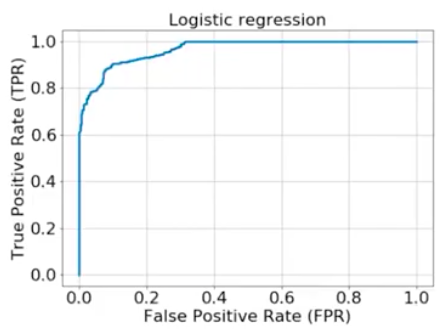
\includegraphics[scale=0.3]{roccurve.png}
\end{figure}
\end{frameex}


\newpage
In high energy physics, we very often plot dependency of \textit{background reduction} from \textit{signal efficiency}. In this case, \textit{signal efficiency} is to be interpreted as the true positive rate and \textit{background reduction} is to be interpreted as one minus the false positive rate. The resulting curves are very similar to the ROC curve.\\

Next, we should comment on the interpretation of the ROC curve. The quality of a classifier is related to \textit{area under the ROC curve}.

\begin{framedef}
We define the quality metric \textit{ROC AUC} to be the \textit{area under the ROC curve}. We note that:
\begin{itemize}
\item ROC AUC $\in [0,1]$.
\item ROC AUC $= 0.5$ corresponds to random guessing.
\item ROC AUC $=1$ means ideal classification.
\item ROC AUC $=0$ also means ideal classification, but for opposite labels!
\end{itemize}

\begin{figure}[H]
\centering
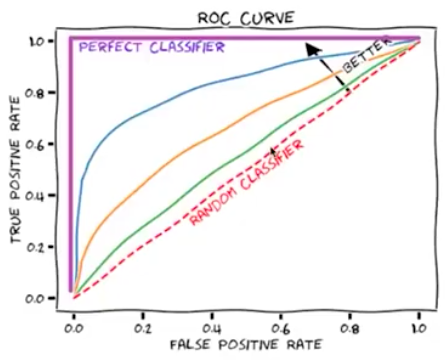
\includegraphics[scale=0.4]{roccurveinterpretation.png}
\end{figure}
\end{framedef}

Similarly to the ROC curve, we can also define a \textit{precision-recall curve} (PR), the curve with coordinates $(\text{Recall}(\mu), \text{Precision}(\mu))$ as the probability threshold $\mu$ is varied. This also induces a quality metric using the area under the curve (PR AUC).

\begin{figure}[H]
\centering
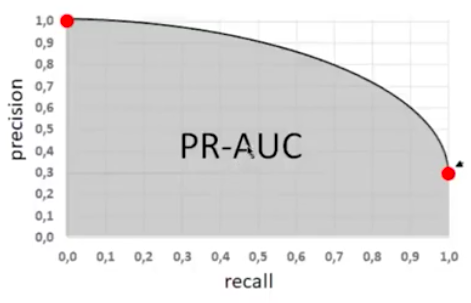
\includegraphics[scale=0.4]{prcurve.png}
\end{figure}



\newpage
\begin{frameex}
We can investigate each of these quality metrics by \textit{fixing a model} but \textit{changing the class balance} in the test sample. Let's choose to make the balances $1:1$, $1:10$ and $10:1$ as shown below:
\begin{figure}[H]
\centering
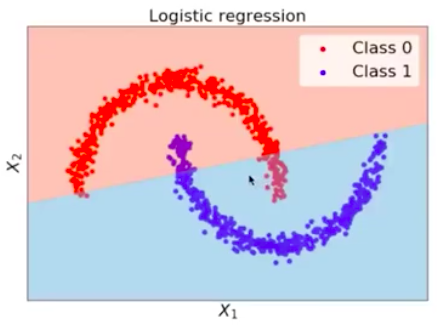
\includegraphics[scale=0.3]{oneoneratio.png}
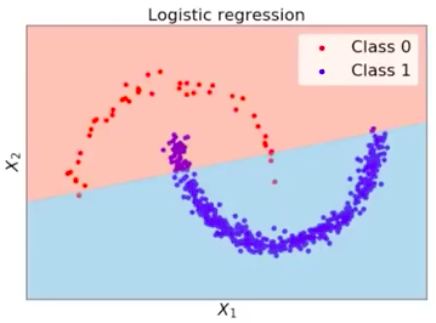
\includegraphics[scale=0.3]{onetenratio.png}
\includegraphics[scale=0.3]{tenoneratio.png}
\end{figure}
The resulting quality metrics are given by:
\begin{figure}[H]
\centering
\includegraphics[scale=0.4]{classifiertable.png}
\end{figure}
With the class balance changing, some metrics change. We note that:
\begin{itemize}
\item Recall and ROC AUC do not change with the class balance changing. This is a general feature.
\item Accuracy did not change with the class balance changing - however, this isn't true in general.
\end{itemize}
\end{frameex}




\newpage
\section{Model tests}

\subsection{Train/test split}
We have already discussed the need for splitting our data into a training set and a test set. This is a quick reminder of how we can use this in regression and classification.

\begin{frameex}
Consider a binary classification problem. We randomly divide our data into two equal samples: \textit{train} and \textit{test}. We use the train sample to fit a classifier. 
\begin{figure}[H]
\centering
\includegraphics[scale=0.4]{classifierexample.png}
\includegraphics[scale=0.4]{fittedclassifier.png}
\end{figure}
Note that in our case, the fitted model has quite an irregular decision boundary - this suggests that some overfitting has taken place, and the model may not be very generalisable.\\

After fitting the model, we can evaluate quality metrics on both the train and test sets. We find:
\begin{figure}[H]
\centering
\includegraphics[scale=0.4]{testtrain.png}
\end{figure}
The values on the training set are greater than on the test set. The reason that this has occurred is that the classifier has learned the training sample specifics, i.e. it has \textit{overfitted}.\\

As a result, the quality metrics are larger on the training set, but since these specifics are \textit{not} properties of the classes, they are not observed in the test sample - thus the classifier makes more mistakes on the test set, and the quality metrics are smaller on that set.\\

As a general rule: the larger differences between the metrics on the train and test set, the greater the extent of model overfitting.
\end{frameex}



\newpage
Let's consider train/test splits in general. We would like to divide our original dataset (written as $(X,y)$ where $X$ is our design matrix and $y$ is our tuple of predictions) into a train set (used to fit and tune a model) and a test set (used to measure the quality of the model). 
\begin{figure}[H]
\centering
\includegraphics[scale=0.4]{traintestsplit.png}
\end{figure}
We can then tune \textit{hyperparameters} in our model, for example coefficients in some regularisation method, refit the model on the training and measure its quality on the test. Overall our aim is to increase quality on the test.\\

How do we come up with a strategy for dividing data between a train and test set? In general we do the following:
\begin{itemize}
\item Data is divided between the train and test \textit{randomly} to ensure distributions on the train and test are similar.
\item Usually we take the train size greater than or equal to the test size. Typical proportions include $1:1$ or $2:1$.
\item The larger the training size, the better the model will fit. However, if the test size is larger, our quality measurements on the test set will be more accurate.
\item The test size can also be \textit{estimated} based on a desired acceptable uncertainty of the quality metrics.
\end{itemize}
In general, a large part of the data is not used for the model fit. This might be crucial for small dataset.\\

Even when we have a train/test split, if we turn our model too long using the same \textit{test} sample, we can find values of the model's hyperparameters such that we \textit{overfit} on the \textit{test} set! To prevent this, we can split our data into \textit{train, validation} and \text{test} sets.
\begin{figure}[H]
\centering
\includegraphics[scale=0.4]{traintestvalidation.png}
\end{figure}
As before, the train set is used to fit and tune the model. The \textit{validation} set is used to measure the quality of the model during its tuning when we are searching for the best hyperparameter values. The \textit{test} set is used only for the final quality measurement (after tuning). This quality is considered the quality of the model.



\newpage
\subsection{Cross-validation methods}
We will now discuss various methods of \textit{cross-validation}. The first we consider is \textit{$k$-folding}. 

\begin{framedef}
In the method of \textit{$k$-folding}, the dataset is split into $k$ parts, or $k$ `folds'. One fold is used to measure quality of the model (as a \textit{validation set}), whilst the other $k-1$ folds are used to train the model. This procedure is repeated $k$ times, and the average quality metric on the validation sets is computed to estimate the final quality; we can also collect the standard deviation of the quality metrics (or different confidence levels for example).
\begin{figure}[H]
\centering
\includegraphics[scale=0.3]{kfolding.png}
\end{figure}
The main disadvantage of this procedure is that it is very time-consuming - it requires fitting the model $k$-times. Typical numbers of folds are around $5$-$10$.
\end{framedef}

A useful modification is \textit{stratified $k$-folding}. This works exactly the same as normal $k$-folding, but when the folds are created, the \textit{same} class balance is used across all folds. This method is useful when we have large class imbalances and small datasets.
\begin{figure}[H]
\centering
\includegraphics[scale=0.3]{stratifiedkfolding.png}
\end{figure}

An extreme case of $k$-folding is \textit{leave one out} cross-validation. This is $k$-folding where the number of folds is equal to the size of the dataset, and can be useful for very small sample sizes.
\begin{figure}[H]
\centering
\includegraphics[scale=0.3]{leaveoneout.png}
\end{figure}
In detail, consider a sample with $N$ objects. For $N$ iterations, remove the $i$th object from the sample, and fit the model using the remaining $N-1$ objects. Using the model, make a prediction for the $i$th object and save it. Collect all predictions and measure the quality of the model.\\

Note that the models from each iteration will be approximately the same (since we hardly change the dataset). Therefore, the predictions will demonstrate a very small variance. \\

Yet another similar approach is \textit{leave $p$ out} cross-validation. Here, we simply remove $p$ randomly selected objects instead of one, for each iteration. As a result, fewer iterations are required.

\begin{figure}[H]
\centering
\includegraphics[scale=0.3]{leavepout.png}
\end{figure}


\minirule

The \textit{bootstrap method} is described as follows:
\begin{itemize}
\item Consider a sample of size $n$ as shown in the figure below. We generate $B$ sets of `bootstrap samples' also of size $n$; these are generated by randomly sampling objects from the original sample \textit{with replacement}. Thus an object can appear in a bootstrap sample several times.
\item For each of the $B$ bootstrap samples, a target is estimated (e.g. if we  wanted to estimate the mean of the whole sample, we could compute the mean on each of the $B$ boostrap sets).
\item Compile a list of the $B$ target estimates. Make further inference from these values, e.g. compute their mean, standard deviation, or even plot their distribution.
\end{itemize}

\begin{figure}[H]
\centering
\includegraphics[scale=0.4]{bootstrap.png}
\end{figure}



\newpage
The bootstrap method can be used for a cross-validation method called \textit{out-of-bag bootstrap}. The method is as follows:
\begin{itemize}
\item Given a dataset of size $n$, we create $B$ random bootstrap samples of size $n$ by sampling \textit{with replacement} as usual. These samples become \textit{training sets}.
\item For each of the $B$ bootstrap samples, determine which elements of the original dataset are not present in the particular sample. These objects comprise \textit{test sets} for each of the corresponding training sets; we can compute required quality metrics on these sets.
\end{itemize}
Once we are done, we can estimate the mean and standard deviation of the quality metrics.

\begin{figure}[H]
\centering
\includegraphics[scale=0.4]{outofbagbootstrap.png}
\end{figure}






\newpage

\subsection{Quality metric uncertainty estimation}
Our goal in this section is to estimate uncertainty of the quality metric on the test set. Again, we can use the bootstrap method:
\begin{itemize}
\item Suppose we are given a model fitted on a training set. Suppose that there are $N$ objects in a corresponding test set.
\item For $i=1,...,B$ bootstrap sample (typically of the order of hundreds or thousands):
\begin{itemize}
\item Sample \textit{with replacement} a subsample with $N$ objects from the test sample.
\item Calculate quality metrics on this subsample.
\end{itemize}
\item Estimate statistics of this metrics, for example \textit{mean}, \textit{variance}, \textit{confidence intervals}.
\end{itemize}
The main advantage of this approach is that it is completely universal - it can be used for any model and any metric. It also does not required fitting the model times.

\begin{frameex}
In the binary classification example before, with model:
\begin{figure}[H]
\centering
\includegraphics[scale=0.4]{fittedclassifier.png}
\end{figure}
applying the bootstrap method gives the following uncertainties:
\begin{figure}[H]
\centering
\includegraphics[scale=0.4]{bootstrapuncertainties.png}
\end{figure}
The means are the same as those computed on the test set, but now we have uncertainties on these values.
\end{frameex}

We can also use cross-validation methods as previously described to estimate the quality metric uncertainties. For example, $k$-folding or out of bag bootstrap can be applied in similar ways - however, these require fitting a model several times.



\newpage
\subsection{Statistical model comparison}
Consider two different models fitted on the same training sample:
\begin{figure}[H]
\centering
\includegraphics[scale=0.4]{statisticalcomparison.png}
\end{figure}
How do we know which model is statistically better? Visually, the model in the left figure has more of a regular separation surface. Additionally, the mean accuracy of the model on the left is higher, but it has a lower uncertainty on accuracy than the model on the right hand side.\\

To distinguish between the models, we use \textit{hypothesis testing}. We have two hypotheses in this case:
\begin{itemize}
\item $H_0$: the models have the same quality (the \textit{null hypothesis}).
\item $H_1$: the models have different qualities.
\end{itemize}
To test whether to reject the null hypothesis $H_0$ or not, we do the following:
\begin{itemize}
\item Select a test statistic, and calculate its value under the null hypothesis.
\item Estimate the $p$-value for the observed statistic value.
\item Compare the $p$-value with the given \textit{significance level}.
\item Based on a decision rule, reject $H_0$ and accept $H_1$ \textit{or} do not reject $H_0$.
\end{itemize}
These steps are illustrated in the following image:
\begin{figure}[H]
\centering
\includegraphics[scale=0.4]{hypothesistesting.png}
\end{figure}


\newpage
Examples of tests and statistics are described as follows. First, consider the \textit{resampled paired $t$-test}:
\begin{itemize}
\item Given two models $A$ and $B$, for $i=1,...,k$:
\begin{itemize}
\item Randomly split the data into training and test samples.
\item Fit the models $A$ and $B$ on the training sample.
\item Compute quality metrics $q_{Ai}$ and $q_{Bi}$ for the models on the test sample.
\end{itemize}
\item Compute the following $t$-statistic with $k-1$ degrees of freedom under the null hypothesis that the models have equal quality:
\begin{equation*}
t = \frac{\overline{q} \sqrt{k}}{\sqrt{\displaystyle \sum_{i=1}^{k} (q_i - \overline{q})^2 / (k-1)}},
\end{equation*} 
where $q_i = q_{Ai} - q_{Bi}$ and $\overline{q} = \displaystyle \sum_{i=1}^{k} q_i$. 
\item Given the estimate $t$-statistic value, we compute the $p$-value for this statistic using \textit{Student's distribution} for $k-1$ degrees of freedom. We compare this $p$-value with the chosen \textit{significance level} (e.g. $\alpha = 0.05$).
\item If the $p$-value is less than $\alpha$, the null hypothesis is rejected. This means that there is a significant difference between the models.
\end{itemize}

\begin{frameex}
For the two models at the start of this section, we can compute the $t$-statistic to be $t = 1.930$. The $p$-value is then given by $0.063$. This is larger than $0.05$, so the null hypothesis is not rejected. The models are \textit{not} significantly different in terms of accuracy.
\end{frameex}

\minirule

Another test is \textit{Dietterich's $5\times2$-fold CV paired test}:
\begin{itemize}
\item Given two models $A$ and $B$, for $i=1,...,5$:
\begin{itemize}
\item Randomly split the data into training and test samples. Fit the models $A$ and $B$ on the training sample. Compute quality metrics $q_{Ai}^{(1)}$ and $q_{Bi}^{(1)}$ for the models on the test sample.
\item \textit{Rotate} the training and test samples: fit the models on the test, compute the metrics $q_{Ai}^{(2)}$ and $q_{Bi}^{(2)}$ on the training sample.
\item Compute the following values:
\begin{equation*}
q_i^{(1)} = q_{Ai}^{(1)} - q_{Bi}^{(1)}, \qquad q_i^{(2)} = q_{Ai}^{(2)} - q_{Bi}^{(2)}, \qquad \overline{q}_i = \frac{q_i^{(1)} + q_i^{(2)}}{2}, \qquad s_i^2 = (q_i^{(1)} - \overline{q}_i)^2 + (q_i^{(2)} - \overline{q}_i)^2.
\end{equation*}
\end{itemize}
\item Then calculate the following $t$-statistic with $5$ degrees of freedom and the null hypothesis that the models $A$ and $B$ have equal qualities:
\begin{equation*}
t = \frac{q_1^{(1)}}{\sqrt{\displaystyle \frac{1}{5} \sum_{i=1}^{5} s_i^2}}.
\end{equation*}
\item Compute the $p$-value for this statistic using Student's distribution for $5$ degrees of freedom. Compare the $p$-value with the chosen significance level $\alpha$. If the $p$-value is less than $\alpha$, the null hypothesis is rejected and there is a significant difference between the two models.
\end{itemize}

\newpage
\begin{frameex}
Applying this test to the above example, we find that $t = 2.073$ and the $p$-value is $0.093$. We see that the null hypothesis is \textit{not} rejected, and again we conclude that the models are not significantly different in terms of accuracy.
\end{frameex}

There are many other available tests, including:
\begin{itemize}
\item Alpaydin's combined $5 \times 2$ CV $F$-test.
\item Cochran's $Q$-test.
\item Friedman's test.
\end{itemize}
However, a detailed discussion is beyond the scope of these lectures.




\newpage
\section{Decision trees}

\subsection{Decision tree training}
Decision trees are a machine learning algorithm for classification and regression. Decision trees themselves predate machine learning, and can are used to make a decision e.g.
\begin{figure}[H]
\centering
\includegraphics[scale=0.4]{decisiontree.png}
\end{figure}
In our case, we would like to build a decision tree for example for classification problems, to decide which class a given element belongs to (hence a decision tree determines a decision boundary).\\

In general, building an optimal decision tree is an NP-complete problem. Therefore, in practice we use a \textit{greedy algorithm} to build a decision tree - on each iteration, we partition the data as if the split was final (we don't think ahead at all). There are two key components:
\begin{itemize}
\item A split criterion to compare different ways to partition the data.
\item A stopping condition to decide when to stop building the tree.
\end{itemize}
Formally:
\begin{framedef}
We define \textit{greedy decision tree learning} as follows. Suppose we are given an input training set $D = \{(x_i,y_i) : i = 1,..., N\}$. For each node in the tree $u$, we write $R_u \subseteq D$ as the data subset associated with this node. To build each $R_u$ we do the following:
\begin{enumerate}[label = (\arabic*)]
\item Set the first node in the tree $R_{\text{start}} = D$ to be equal to the whole dataset.
\item Given $R_u$ left unsplit and not a leaf, we greedily split $R_u$ into $R_l$ and $R_r$ given by:
\begin{equation*}
R_l(j,t) = \{\vec{x} \in R_u : x^j \leq t\}, \qquad R_r(j,t) = \{\vec{x} \in R_u : x^j > t\},
\end{equation*}
where $j$ is a particular feature, optimising a given loss $Q(R_u,j,t)$ over $(j,t)$.
\item If a stopping criterion is satisfied for $u$, declare it a \textit{leaf} of the true.
\item If not, create an internal node $u$ corresponding to the predicate $x^j \leq t$ and repeat from Step 2 for $R_u = R_l(j,t)$ and $R_u = R_r(j,t)$. 
\end{enumerate}
\end{framedef}

\newpage
A good split at any point in the building of a decision tree is one that maximises \textit{purity}; i.e. objects in the split are as uniform as possible:

\begin{figure}[H]
\centering
\includegraphics[scale=0.3]{goodsplit.png}
\end{figure}

We can formalise the purity by carefully discussing the loss function $Q(D,j,t)$ above. Recall that $R_u$ is the subset of $D$ corresponding to the node $u$. With the current split, let $R_l \subseteq R_u$ go left and $R_r \subseteq R_u$ go right. We choose a predicate to maximise:
\begin{equation*}
Q(R_u, j, t) = H(R_u) - \frac{|R_l|}{|R_u|} H(R_l) - \frac{|R_r|}{|R_u|} H(R_r),
\end{equation*}
where $H(R)$ is some impurity criterion. Generally, we take:
\begin{equation*}
H(R) = \min_{c \in \mathcal{Y}} |R|^{-1} \sum_{(x_i,y_i) \in R} \mathcal{L}(y_i, c),
\end{equation*}
where $\mathcal{L}$ is a loss function, penalising wrong predictions.

\begin{frameex}
Some examples of impurity criterion include:
\begin{itemize}
\item For regression, we might choose MSE:
\begin{equation*}
H(R) = \min_{c \in \mathcal{Y}} |R|^{-1} \sum_{(x_i,y_i) \in R} (y_i - c)^2.
\end{equation*}
This is minimised by $c = |R|^{-1} \displaystyle \sum_{(x_j,y_j) \in R} y_j$, which makes the impurity the variance of the target.
\item For classification, we can enumerate $\mathcal{Y} = \{y_1,...,y_N\}$. We then let:
\begin{equation*}
p_k = |R|^{-1} \sum_{(x_i,y_y) \in R} 1_{\{y_i = y_k\}}
\end{equation*}
be the share of examples belonging to the $k$th class.\\

We could choose the impurity to be the \textit{miss rate} (inaccuracy):
\begin{equation*}
H(R) = \min_{c \in \mathcal{Y}} |R|^{-1} \sum_{(x_i,y_i) \in R} 1_{\{y_i \neq c\}}.
\end{equation*}
We could also choose the impurity to be the \textit{Gini index}:
\begin{equation*}
H(R) = \sum_{k=1}^{N} p_k(1-p_k).
\end{equation*}
Finally, we could choose the impurity to be the \textit{cross-entropy}:
\begin{equation*}
H(R) = -\sum_{k=1}^{N} p_k \log(p_k).
\end{equation*}
\end{itemize}
\end{frameex}



\newpage
\subsection{Stopping rules for decision tree learning}
What will happen if we build a decision tree to minimise the impurity to the greatest possible extent? The tree will be built until all leaves are $100$\% pure, with some leaves only containing a single example. This corresponds to a \textit{dramatic overfitting}. For example: 

\begin{figure}[H]
\centering
\includegraphics[scale=0.4]{decisiontreeoverfitting.png}
\end{figure}

Clearly we need to know when to stop the training to avoid overfitting. There are multiple choices available:
\begin{itemize}
\item Impose a maximum tree depth.
\item Impose a minimum number of objects in a leaf.
\item Impose a maximum number of leaves in a tree.
\item Stop if all objects fall into the same leaf.
\item Constrain \textit{quality improvement} (stop when improvement gains drop below a defined threshold).
\end{itemize}
There is no general way to select the best choice. It is typically decided by exhaustive search and cross-validation.

\minirule

A useful technique that can help to avoid overfitting is \textit{decision tree pruning}. 
\begin{figure}[H]
\centering
\includegraphics[scale=0.4]{pruning.png}
\end{figure}
We train a very large tree (effectively overfitting the training set), then remove the least important nodes. This often leads to better result than simply training a small tree.\\

The reason why is as follows. When we build a tree, we use a greedy algorithm - we never look ahead or plan smart moves. In particular, pruning allows us to recover some of this missing foresight.









\newpage
\part{Introduction to neural networks}
\hrule
\noindent \\
\section{Feature engineering, importance and selection}


\subsection{Feature engineering}
\begin{frameex}
Consider a binary classification problem in 2D with a logistic regression classifier:
\begin{figure}[H]
\centering
\includegraphics[scale=0.4]{circles.png}
\end{figure}
The classes are concentric circles, and the classifier \textit{cannot} separate them using only the input features $X_1, X_2$ - they are not linearly separable.\\

Let's create the new feature $X_3 = X_1^2 + X_2^2$. This feature helps to separate the circles by a straight line. Now, logistic regression can solve the classification problem ideally using all three features $X_1, X_2$ and $X_3$. 

\begin{figure}[H]
\centering
\includegraphics[scale=0.4]{circles2.png}

\end{figure}
\end{frameex}

The above example shows how `feature engineering' can improve the predictions of linear models.




\newpage
\begin{frameex}
Consider another example where the two classes are separated by the surface $X_2 - X_1 = 0$. 
\begin{figure}[H]
\centering
\includegraphics[scale=0.4]{treeline.png}
\end{figure}
These classes are linearly separable, and can be found using a logistic regression model.\\

However, the problem is difficult to solve with a decision tree classifier (as shown above - it splits input feature space with \textit{rectangles}). It requires larger depth of the tree to separate the classes properly.\\

If we introduce the new feature $X_3 = X_2 - X_1$, we help the classifier. Now the classes can be separated using just one predicate $X_3 > 0$. It requires a decision tree with depth $1$ to solve the problem ideally.

\begin{figure}[H]
\centering
\includegraphics[scale=0.4]{treeline2.png}
\end{figure}
\end{frameex}

These two examples show that creating new features can:
\begin{itemize}
\item Improve the quality of a model.
\item Reduce the complexity of a model (see the shorter decision tree in the second example).
\item Speed up model training (due to reduced complexity).
\item Reduce dimensionality of a problem by removing less informative features (e.g. $X_1, X_2$ in previous examples - these can be removed without losing the model's qualtiy!).
\end{itemize}




\newpage
But how do we choose which new features will be useful? There are some general principles:
\begin{itemize}
\item Use any information about the problem we have. In the above examples the information we had was the shape of the classes and the border between them.
\item Create features with physical meaning (e.g. $\sqrt{X_1^2 + X_2^2}$ is radius). For example in high energy physics, we might like to use momenta, mass, angles, etc.
\item Remove limitations of a model (like with the decision tree in example 2).
\end{itemize}

Given an initial set of input features $X_1,...,X_n$, typical feature combinations include:
\begin{itemize}
\item Powers and products, e.g. $X_i^p$, $X_1X_2$.
\item Sums and differences of squares, e.g. $X_1^2 \pm X_2^2$.
\item Sums and differences, e.g. $X_1 \pm X_2$.
\item Sum and difference quotients, e.g.
\begin{equation*}
\frac{X_1 \pm X_2}{X_1 \mp X_2}
\end{equation*}
\item More complicated functions, e.g.
\begin{equation*}
\sin(X_1), \qquad \cos(X_1).
\end{equation*}
\end{itemize}

\minirule

\subsection{Feature importance}
Let us try to address the problem of which features are important more carefully.\\

A dataset can have a lot of features, but not all features are equally useful for a given regression or classification task. Some of them are more informative than others. Consider the example below:

\begin{figure}[H]
\centering
\includegraphics[scale=0.4]{uselessfeature.png}
\end{figure}

We see that the feature $X_1$ is completely uninformative for the classification problem, and can be skipped. We can easily spot this from the plot of the data, but how can we do this in multi-dimensional cases? Our goal should be to measure the importance of each feature in the general case somehow.






\newpage
There are several different methods to achieve this:
\begin{itemize}
\item Correlations between features and target values.
\item Probabilistic distances.
\item Decision tree-based feature importance.
\item Linear model-based feature importances.
\end{itemize}
Finally we will consider a completely general algorithm which can be applied for any classification or regression problem.\\

We begin with correlations:
\begin{framedef}
Let $f$ be a feature and let $y$ be a target. Denote by $f_i$ the value of the feature for the $i$th object in a dataset, and by $y_i$ the value of the target for the $i$th object in a dataset (this corresponds to labels $0$ or $1$ for example in a binary classification problem, or to the target values in a regression problem). We define the \textit{Pearson correlation coefficient} by:
\begin{equation*}
\rho(f, y) = \frac{\displaystyle \sum_{i} (f_i - \overline{f})(y_i - \overline{y})}{\sqrt{\displaystyle \sum_{i} (f_i - \overline{f})^2 \sum_{i} (y_i - \overline{y})^2}},
\end{equation*}
where $\overline{f}$ is the mean of the feature over the dataset, and $\overline{y}$ is the mean of the target values over the dataset. 
\end{framedef}

This measurement of feature importance is very easy to compute, but captures only linear dependencies in dataset:

\begin{figure}[H]
\centering
\includegraphics[scale=0.3]{correlationcoefficient.png}
\end{figure}

Another simple approach is based on \textit{probabilistic distance}:
\begin{framedef}
Let $f$ be a feature, and let $y$ be a target taking values $0$ or $1$ (i.e. a binary classifier).

\begin{figure}[H]
\centering
\includegraphics[scale=0.3]{featureprobabilities.png}
\end{figure}

We define the \textit{total variation} between the probability distributions $\mathbb{P}(f | y=0)$ and $\mathbb{P}(f | y = 1)$ to be:
\begin{equation*}
\textrm{Imp}(f) = \int \left| \mathbb{P}(f | y = 1) - \mathbb{P}(f | y =0) \right|\ df.
\end{equation*}
There are other methods of measuring the distance between probability distributions - we will consider these later in the school. 
\end{framedef}



\newpage
Another approach is based on \textit{decision trees}. Recall from the previous lectures that a decision tree is a binary tree where each node $t$ has two children. Each node uses one feature to make a split into the two children notes. For each node, we compute the number of objects $n_t$ which satisfy the criteria in the node; then for each node we can compute \textit{impurity} functions $I(t)$ (e.g. Gini, cross-entropy, MSE) for the node. 

\begin{figure}[H]
\centering
\includegraphics[scale=0.4]{featuretree.png}
\end{figure}

\begin{framedef}
Let $T(f)$ be the set of all nodes which use feature $f$ to make a split. Then feature importance can be estimated by:
\begin{equation*}
\textrm{Imp}(f) = \sum_{t \in T(f)} n_t \Delta I(t),
\end{equation*}
where the \textit{information} $\Delta I(t)$ contained in the node $t$ is defined by:
\begin{equation*}
\Delta I (t) = I(t) - \sum_{c \in \textrm{children}(t)} \frac{n_c}{n_t} I(c).
\end{equation*}
\end{framedef}
This statistic is one of the most popular and important for feature estimation. It takes into account dependencies between different input features, and can capture complicated dependencies between features and the target. It is also implemented in almost all decision tree libraries.\\

Another method is \textit{linear-model based}.
\begin{framedef}
Consider a linear model with regularisation (e.g. an $L1$ or $L2$ penalty). The model makes predictions:
\begin{equation*}
\hat{y} = w_0 + w_1 f_1 + w_2 f_2 + \cdots + w_k f_k.
\end{equation*}
If features are normalised (have the same ranges, e.g. by scaling), the feature importance of $f_i$ is defined to be equal to:
\begin{equation*}
\textrm{Imp}(f_i) = |w_i|.
\end{equation*}
\end{framedef}
This method is very simple, but has the same limitations as Pearson correlation - it cannot capture complicated dependencies.



\newpage
Now let's consider a completely general approach. Suppose we have a model used for classification or regression.
\begin{itemize}
\item We train the model to some training set.
\item We calculate the quality measure $Q_0$ on some validation set.
\item For a given feature $f$, we:
\begin{itemize}
\item Replace the given values of this feature with random values from the same distribution (for example, you can perform random shuffling of the value of the feature). 
\begin{figure}[H]
\centering
\includegraphics[scale=0.4]{randomshuffle.png}
\end{figure}
\item Compute the new quality measure $Q_f$ on the validation set, and estimate the feature importance as the difference between the initial and current quality metric values:
\begin{equation*}
\textrm{Imp}(f) = Q_0 - Q_f.
\end{equation*}
\end{itemize}
\end{itemize}

This is the most powerful method for computing feature importance. It can capture complicated dependencies, and works for any model - e.g. neural networks, which we shall see soon.\\

There is a slight modification to this method which also works:
\begin{itemize}
\item We train the model on the \textit{full set of features} (as normal)
\item We calculate the quality measure $Q_0$ on some validation set.
\item For a given feature $f$, we:
\begin{itemize}
\item Remove the feature $f$ from the dataset, then \textit{refit the model without this feature}. 
\begin{figure}[H]
\centering
\includegraphics[scale=0.4]{featureremoval.png}
\end{figure}
\item Compute the new quality measure $Q_f$ on the validation set, and estimate the feature importance as the difference between the initial and current quality metric values:
\begin{equation*}
\textrm{Imp}(f) = Q_0 - Q_f.
\end{equation*}
\end{itemize}
\end{itemize}
The advantage of this approach is that it estimates the feature importances more precisely, and works better for highly correlated input features. However, it requires refitting the model several times - this might be difficult for large models and datasets.\\

There are many other approaches to estimate feature importance which we don't have time to discuss here - for example the method of \textit{Shapley values}, which has a Python implementation.





\newpage
\subsection{Feature selection}
The goal of \textit{feature selection} is to reduce the number of features with minimal loss of model quality. For example, we might want to keep the best $K$ of $D$ features, or we might want to remove as many features as possible but keeping the quality $Q \geq Q_{\text{min}}$ for some $Q_{\text{min}}$. 
\begin{figure}[H]
\centering
\includegraphics[scale=0.3]{featureselection.png}
\end{figure}

Three of the most popular methods are the \textit{filter method}, \textit{embedded methods} and \textit{recursive feature elimination}.

\begin{framedef}
The \textit{filter method} involves estimating the importance of individual features $\textrm{Imp}(f_1), \textrm{Imp}(f_2), ..., \textrm{Imp}(f_D)$ via some method (e.g. correlation, probability distance). We then simply select the required number of features with the highest importances.
\end{framedef}

This is simple it implement and is quite fast. However, it is bad for highly correlated features, since it may take many redundant features.

\begin{framedef}
An \textit{embedded method} selects features based on the feature importance of a model.
\begin{itemize}
\item In a linear model, an embedded method selects the best features using the weights of the model (as above).
\item For a decision tree, the best features are selected using their decision tree importance (as above).
\end{itemize}
\end{framedef}
Embedded methods is widely used and take into account correlation between features.\\

Finally, we have \textit{recursive feature elimination}. Uninformative features are removed one by one, based on deleting the least important feature at each step. 

\begin{figure}[H]
\centering
\includegraphics[scale=0.3]{recursivefeature.png}
\end{figure}

The steps are as follows:
\begin{itemize}
\item Train a model on the full set of features, and estimate the importance of each feature based on the model.
\item Remove the least importance features (or several features).
\item Repeat until we have the desired number of features remaining.
\end{itemize}
In combination with the general method for feature importance estimation, this is one of the most powerful methods for feature selection. It is applicable to any regression or classification problem.






\newpage
\section{Clustering}

So far, we have studied classification and regression models. These are models of `supervised learning' where we know exactly what to predict - class labels for classification or real labels for regression.\\

In this section, we will discuss \textit{clustering}, where we do not have any target values for predictions. Therefore clustering is a topic of `unsupervised machine learning'.

\minirule

\subsection{Clustering vs classification}
Consider a binary classification problem, where we have object features $X$ and class labels $y \in \{0,1\}$. A classifier learns a decision rule $f$, so that $f(X) \approx y$. The trained classifier predicts class labels for the new objects.
\begin{figure}[H]
\centering
\includegraphics[scale=0.4]{supervisedclassifier.png}
\end{figure}
In clustering, we don't have class labels $y$. The goal is to divide all objects into separate groups using only object features $X$ - these groups are called \textit{clusters}. 
\begin{figure}[H]
\centering
\includegraphics[scale=0.4]{clusterclassification.png}
\end{figure}
We would like to cluster the objects such that \textit{objects inside clusters are similar}, and \textit{objects from different clusters are dissimilar}. In the above figure, `similarity' can be defined as proximity to the other objects.\\

Most clustering algorithms are based on the following assumptions:
\begin{itemize}
\item Objects form \textit{dense} clusters. This means that the object density inside one cluster is larger than between the clusters.
\item Objects from one cluster are somehow similar, whilst objects from different clusters are somehow dissimilar. Often similarity between objects is based on `distance' between them.
\item Distances between neighbours within one cluster are smaller than between objects from different clusters.
\end{itemize}



\newpage
\subsection{$K$-means}
The most popular clustering approach is the approach of \textit{$K$-means}. We develop intuition for this approach as follows.\\

We suppose that each cluster is represented by a \textit{centre}. All objects are assigned to a cluster according to the closest centre. The goal of the problem is therefore to \textit{find centres that form the most compact clusters}.
\begin{figure}[H]
\centering
\includegraphics[scale=0.4]{kmeans.png}
\end{figure}

Let's define some notation which we will use throughout this section. Consider a sample with $N$ objects, written $\{x_n\}_{n=1}^{N}$ (where $x_n$ denotes a tuple of features). We will search for $K$ clusters with centres $\{\mu_1,...,\mu_K\}$. The criterion to find the best centres is minimising the \textit{within-cluster distance} over $\mu_1,...,\mu_K$:
\begin{equation*}
Q = \sum_{n=1}^{N} \min_{k} \rho(x_n,\mu_k).
\end{equation*}
Each object is then assigned to a cluster $z_n \in \{1,2,...,K\}$ via:
\begin{equation*}
z_n = \underset{k}{\textrm{argmin}}\ \rho(x_n, \mu_k).
\end{equation*}
A general algorithm that achieves this is as follows (called the \textit{$K$-centroid algorithm}):
\begin{enumerate}[label = (\arabic*)]
\item Initialise the centres $\mu_1,...,\mu_K$ by randomly selecting $k$ objects from the sample.
\item Assign each object of the sample to the nearest centre:
\begin{equation*}
z_n = \underset{k}{\textrm{argmin}}\ \rho(x_n, \mu_k),
\end{equation*}
where $\rho$ is the `distance' between two objects.
\item Update the centres by minimising the within cluster distance, i.e. determining:
\begin{equation*}
\mu_k = \underset{\mu}{\textrm{argmin}} \sum_{n : z_n = k} \rho(x_n, \mu).
\end{equation*}
\item If the algorithm has not converged to within some tolerance, go to Step 2 and repeat. Otherwise return $z_1,...,z_N$. 
\end{enumerate}


\newpage
The above algorithm can use difference distances $\rho$:
\begin{framedef}
If $\rho(x_n, \mu_k) = ||x_n - \mu_k||_2^2$, the above algorithm is called the \textit{$K$-means algorithm}. If $\rho(x_n, \mu_k) = ||x_n - \mu_k||_1$, the above algorithm is called the \textit{$K$-medians algorithm}.
\end{framedef}

The $K$-means algorithm can be implemented efficiently as follows:
\begin{enumerate}[label = (\arabic*)]
\item Initialise the centres $\mu_1,...,\mu_K$ by randomly selecting $k$ objects from the sample.
\item Assign each object of the sample to the nearest centre:
\begin{equation*}
z_i = \underset{j \in \{1,2,...,K\}}{\textrm{argmin}}\ ||x_i - \mu_k||_2^2.
\end{equation*}
\item Update the centres using the following minimisation (this choice minimises the within-cluster distance):
\begin{equation*}
\mu_j = \frac{\displaystyle \sum_{n=1}^{N} 1_{\{z_n = j\}} x_i}{\displaystyle \sum_{n=1}^{N} 1_{\{z_n = j\}}}.
\end{equation*}
\item If the algorithm has not converged to within some tolerance, go to Step 2 and repeat. Otherwise return $z_1,...,z_N$. 
\end{enumerate}
Below is an example of the convergence of the algorithm:
\begin{figure}[H]
\centering
\includegraphics[scale=0.4]{kmeansconvergence.png}
\end{figure}

Let's discuss the properties of the $K$-means algorithm in more detail:
\begin{itemize}
\item \textbf{Initialisation.} The centres $\{\mu_k\}_{k=1}^{K}$ are usually initialised randomly from training objects. The number of clusters (and centres) $K$ is usually fixed.
\item \textbf{Convergence criteria.} There are various methods we could use to check for convergence. For example, we could set some limit on the number of iterations of the algorithm, we could demand that the centres stop changing significantly within some tolerance, or we could ask that the cluster assignments $\{z_n\}_{n=1}^{N}$ stop changing.
\item \textbf{Solution.} The solution depends on the starting positions of the centres. In particular, this means that the algorithm is sensitive to outliers, and may create single-object clusters. To prevent this it is recommended to run the algorithm with several different initialisations, and select the solution with the minimal within-cluster distance $Q$. 
\end{itemize}



\newpage
Now we understand how $K$-means works, we can ask some interesting questions about it. For example - how do we know how many clusters $K$ to split the data into? Using the wrong number of clusters can lead to bad results, e.g.
\begin{figure}[H]
\centering
\includegraphics[scale=0.4]{wrongclusters.png}
\end{figure}
Let $Q^{(K)}$ denote the within-cluster distances for each possible number of clusters $K$,
\begin{equation*}
Q^{(K)} = \sum_{n=1}^{N} ||x_n - \mu_{z_n}||_2^2.
\end{equation*}
We wish to minimise this over $z_1,...,z_N, \mu_1,...,\mu_K$.\\

The dependency of $Q^{(K)}$ on $K$ is demonstrated in the figure below for the above example.
\begin{figure}[H]
\centering
\includegraphics[scale=0.4]{elbow.png}
\end{figure}
The dependence has an `elbow' at the optimal number of clusters, $K=5$. Let's try to formalise this notion.\\

We define the function $D(K)$ by:
\begin{equation*}
D(K) = \frac{|Q^{(K+1)} - Q^{(K)}|}{|Q^{(K)} - Q^{(K-1)}|}.
\end{equation*}
This function takes its smallest value for the optimal number of clusters.

\begin{figure}[H]
\centering
\includegraphics[scale=0.4]{optimalclusters.png}
\end{figure}




\newpage
\subsection{Quality metrics}
Now we know one clustering algorithm. How do we measure the quality of a clustering algorithm?\\

There are two kinds of quality metrics for clustering models: \textit{supervised} and \textit{unsupervised}.
\begin{itemize}
\item \textit{Supervised} quality metrics are based on the ground truth of the object labels. They are invariant to cluster naming. Unfortunately, very often the true labels are unknown and hence it is impossible to use these metrics in this case.
\item \textit{Unsupervised} quality metrics are based on intuition about `good' clusters. They assume that objects from the same cluster are similar to one another, and objects from different clusters are dissimilar to one another.
\end{itemize}

One supervised quality metric is the \textit{Rand index}:
\begin{framedef}
The \textit{Rand index} is the supervised quality metric defined as:
\begin{equation*}
\text{RI} = \frac{\text{TP} + \text{TN}}{\text{TP} + \text{TN} + \text{FP} + \text{FN}}.
\end{equation*}
Here, TP denotes \textit{true positives}, the number of pairs in the same cluster in predictions and the ground truth. TN denotes \textit{true negatives}, the number of pairs from different clusters in predictions and the ground truth. FP denotes \textit{false positives}, the number of pairs in the same cluster in predictions, but from different clusters in the ground truth. FN denotes \textit{false negatives}, the number of pairs in the same cluster in the ground truth, but from different clusters in predictions.
\end{framedef}
The Rand index takes values in $[0,1]$, where $1$ means perfect clustering. It is similar to accuracy score, but for pairs.\\

A slight modification is:
\begin{framedef}
The \textit{adjusted Rand index} (ARI) is defined by:
\begin{equation*}
\text{ARI} = \frac{\text{RI} - \text{RI}_{\text{expected}}}{\text{RI}_{\text{max}} - \text{RI}_{\text{expected}}}.
\end{equation*}
The expected Rand index is taken by averaging the Rand index over all possible object assignments to the clusters. \\

The ARI has a value close to $0$ for random labelling, independently of the number of clusters and sample, and exactly $1$ when the clustering is ideal.
\end{framedef}

As we have just seen Rand index is very similar to accuracy score. We can compute similar metrics like precision, recall, or $F_1$-score in the same sorts of ways by just considering pairs.\\

One of the most popular unsupervised metrics is the \textit{silhouette metric}:
\begin{framedef}
The \textit{silhouette metric} is defined by:
\begin{equation*}
\textrm{Silhouette} = \frac{1}{N} \sum_{i=1}^{N} \frac{d_i  - s_i}{\max(d_i ,s_i)}
\end{equation*}
where $s_i$ is the mean distance between the $i$th object and all objects in the same cluster, and $d_i$ is the mean distance between the $i$th object and all objects in the nearest (distinct) cluster. It is based on the idea that objects in one cluster should be closer to one another than objects in different clusters.
\end{framedef}

\begin{frameex}
Consider clustering of the following data with $K$ clusters:
\begin{figure}[H]
\centering
\includegraphics[scale=0.4]{clusterquality1.png}
\end{figure}
The quality metrics for the clustering are given below:
\begin{figure}[H]
\centering
\includegraphics[scale=0.4]{clusterquality2.png}
\end{figure}
Each quality metric predicts the optimum number of clusters is $K=5$.
\end{frameex}










\end{document}
